\documentclass[11pt,twoside,ngerman,a4paper]{article}
\usepackage{graphicx}
\usepackage{float}
\usepackage[T1]{fontenc}
\usepackage{mathpazo}
%\usepackage{xcolor}
\usepackage{verbatim} %Comments
\usepackage{amsmath}
\usepackage{setspace}
\usepackage[ngerman=ngerman-x-latest]{hyphsubst}
\usepackage[font=small,labelfont=bf]{caption}
%\usepackage[lining,scaled=.95]{ebgaramond} % The default is oldstyle numbers.
%% I have set the numbers to be lining to display lining numbers as well as
%% oldstyle numbers
\usepackage[utf8x]{inputenc}
\usepackage[]{geometry}
\geometry{verbose,tmargin=3.3cm,bmargin=6.6cm,lmargin=4.6cm,rmargin=2.3cm,headheight=2cm,footskip=3cm}
\usepackage{fancyhdr} % für eigene Kopf- und Fußzeilen
\pagestyle{fancy} %eigener Seitenstil
\fancyhf{} %alle Kopf- und Fußzeilenfelder bereinigen
%linke Seite (gerade Seitenzahl)
\fancyhead[ERL]{Koptertracking mittels TLD} % links
\fancyhead[ERC]{} % zentriert
\fancyhead[ERR]{} % rechts
%rechte Seite (ungerade Seitenzahl)
\renewcommand{\sectionmark}[1]{\markboth{#1}{}} % Vorbereitung der Kapitelausgabe
\fancyhead[ORL]{} % links
\fancyhead[ORC]{} % zentriert
\fancyhead[ORR]{ \textit{\leftmark}} % rechts - Ausgabe des Kapitels
%\renewcommand{\headrulewidth}{0.4pt} %obere Trennlinie
\fancyfoot[C]{\thepage} %Seitennummer
\renewcommand{\footrulewidth}{0.4pt} %untere Trennlinie
%Abbildungsunterschrift ändern
\renewcommand{\captionfont}{\small\slshape}
\renewcommand{\figurename}{Abbildung}
\renewcommand{\thefigure}{\arabic{section}.\arabic{figure}}
\makeatletter \@addtoreset{figure}{section} \makeatother
%\PassOptionsToPackage{normalem}{ulem}
%\usepackage{microtype}
%\usepackage[english, ngerman]{babel}
\usepackage[linesnumbered,ruled,vlined]{algorithm2e}
% \usepackage{algorithm}
% \usepackage{algorithmic}
% \usepackage{algpseudocode}
% Ändern der automatischen Überschriften
\renewcommand{\listfigurename}{Liste der Abbildung}
\renewcommand{\contentsname}{Inhaltsverzeichnis}
\renewcommand{\abstractname}{Abstrakt}
\sloppy
%\usepackage[options]{package}

\begin{document}
	\cleardoublepage % -*- root: diplomarbeit.tex -*-
\thispagestyle{empty}
\hspace{20cm}
\vspace{-2cm}

\begin{figure}[H] \hspace{11cm}
  \includegraphics[width=3.2 cm]{../pictures/HU_Logo}
\end{figure}

\begin{center}
  \vspace{0.5 cm}
  \huge{\bf Koptertracking mittels TLD} \\ % Hier fuegen Sie den Titel Ihrer Arbeit ein.
  \vspace{1.5cm}
  \LARGE  Diplomarbeit \\ % Geben Sie anstelle der Punkte an, ob es sich um eine
   %Diplomarbeit, eine Masterarbeit oder eine Bachelorarbeit handelt.
  \vspace{1cm}
  \Large zur Erlangung des akademischen Grades \\
  Diplominformatiker\\ 
  \vspace{2cm}
  {\large
    \bf{
      \scshape
      Humboldt-Universit\"at zu Berlin \\
      Mathematisch-Naturwissenschaftliche Fakult\"at II \\
      Institut f\"ur Informatik\\
    }
  } 
  % \normalfont
\end{center}
\vspace {1cm}% gegebenenfalls kleiner, falls der Titel der Arbeit sehr lang sein sollte
%{3.2 cm} bei Verwendung von scrreprt, gegebenenfalls kleiner, falls der Titel der Arbeit sehr lang sein sollte
{\large
  \begin{tabular}{llll}
    eingereicht von:    & Ronald Klaus && \\ % Bitte Vor- und Nachnamen anstelle der Punkte eintragen.
    geboren am:         & 5. August 1980 && \\
    in:                 & Hennigsdorf && \\
    &&&\\
    Gutachter(innen): & ... && \\
          & ... && \\% Bitte Namen der Gutachter(innen) anstelle der Punkte eintragen
         % bei zwei männlichen Gutachtern kann das (innen) weggestrichen werden
    &&&\\
    eingereicht am:     & \dots\dots  
    \hspace{3cm} 
    verteidigt am: & \dots\dots \\
  \end{tabular}
} % Deckblatt
	\cleardoublepage % -*- root: diplomarbeit.tex -*-
\begin{abstract}
\begin{singlespace}
In dieser Arbeit wird ein Tracking-Detection-Algorithmus hinsichtlich seiner Eignung für das Finden und Verfolgen von Flugroboter, wie Quadro- und Hexakopter, untersucht. Im Detail besteht die Aufgabe, dass ein solcher Roboter ausgestattet mit einer Kamera, visuellen Informationen für das Finden eines anderen Roboters verarbeitet. 

Der untersuchte Ansatz TLD - Tracking Learning Detection \cite{TLD} ist ein semi-automated single-target tracking-Algorithmus. Das single-target tracking schätzt in einer Sequenz von Bildern $I_{0},\dots,I_{m}$ den Status $x_{k}$ eine Objekts im Bild $I_{k}$ \cite{key-7}. Der semi-automated-Ansatz bezieht sich auf die Initialisierung des Trackens. Im Gegensatz zum automated tracking, in dem der Tracker mittels bereits bestehende Informationen initialisiert wird, und dem manual tracking, bei dem eine Nutzerinteraktion in jedem Bild nötig ist, wird im semi-automated-Tracking ein eine Nutzereingabe für die erste Objektdefinition benötigt.

Für eine erfolgreiche Abreitsweise jedes Trackers, egal welchen Ansatz im zugrunde liegt, sind zwei Anforderungen essentiell: Genauigkeit und Robustheit \cite{key-8}. Beide sind jedoch, bezogen auf die Möglichkeiten zur Optimierung, gegensätzlich. Die Genauigkeit wird vor allem dadurch erreicht wird, dass der Suchradius des Objekts im Folgebild möglichst gering ist, um eine Fehlerfunktion zu minimieren. Zur Optimierung der Robustheit und damit die Reaktion auf eventuelle Änderungen der Lichtverhältnisse oder Bewegungen des Objekts, sollte gerade ein großer Radius zur Suche genutzt werden, damit das Objekt beispielsweise durch eine schnelle Bewegung nicht aus dem Suchfeld verschwindet. Damit muss ein Mittelweg gefunden werden, da eine gleichzeitige Optimierung beider Anforderungen nicht möglich ist.

Typischerweise ist das Finden und Verfolgen von Objekten mit einer nicht-statitischen Kamera in der ``realen'' Welt eines der herausfordernsten Problemstellungen der Computer Vision, da die Umwelt einen großen Einfluss auf die Qualität der visuellen Daten hat. Lichtverhältnisse variieren, eine Fülle anderer Objekte hat eventuell große Ähnlichkeit zum gesuchten Objekt haben, komplexe und nichtstatische Strukturen wie Bäume erschweren das Separieren. Zusätzlich ist definiert, dass das Objekt, in diesem Fall der Kopter, keinerlei Markierungen in Form von farbigen Markern oder speziellen, eindeutigen Mustern erhält.
\end{singlespace}
\end{abstract} 	% Abstract
	\begin{onehalfspace}
	% \begin{singlespace}
		\cleardoublepage \listoffigures % Abbildungsverzeichnis
		\cleardoublepage \listofalgorithms % Algorithmenverzeichnis
		\setcounter{tocdepth}{2}
		\cleardoublepage \tableofcontents  % Inhaltsverzeichnis
		\cleardoublepage
	% \end{singlespace}
	% \begin{onehalfspace}
		\cleardoublepage % -*- root: diplomarbeit.tex -*-
\section{Einleitung}
\textbf{Computer Vision}, das machinelle Sehen, ist eine große Herausforderung in der Bildverarbeitung und Feld intensiver Forschung. Die zunehmende Leistungsfähigkeit der Rechner und verbesserte Qualität auch preiswerter Kameratechnik in den letzten Jahren intensivieren die Bestrebungen auf diesem Gebiet zusätzlich. Die dadurch entstandenen Ansätze, Modelle und Methoden haben längst in vielen Bereichen des Alltags Einzug gehalten. Kaum ein Auto wird ohne ``intelligente'' Sensorik ausgestattet und unterstützt den Fahrer beispielsweise durch Lesen von Straßenschildern, Erkennen von Fahrbahnmarkierungen sowie Fußgängern oder andere Verkehrsteilnehmern \cite{PED}. Die Industrie nutzt computergesteuerte Auswertungen von Kamerabildern zur Qualitätssicherung von Bauteilen wid zum Beispiel Displays \cite{LCD}. In der Medizin helfen computergestützte visuelle Verfahren bei der Analyse von Bilddaten und unterstützen so die Diagnostik \cite{MIP}. Und nicht zuletzt bildet die Auswertung von Kameradaten auch im Forschungsbereich der Robotik oft die Grundlage für viele Unterschiedliche Anwendungen. Die Aufgaben, die an den Bereich Computer Vision gestellt werden, sind somit sehr vielfältig.

Diese Arbeit behandelt einen speziellen Teilbereich des machinellen Sehens: das Finden und Verfolgen von Objekten. Ein definiertes Objekt, das in einer bestimmten Art und Weise repräsentiert ist, soll somit in einem Bild gefunden (Detection) und verfolgt (Tracking) werden. Da noch nicht verstanden ist, wie z.B. das menschliche Gehirn visuelle Daten zur Erkennung von ``gelernten'' Objekten verarbeitet, ist eine Adaption auf Computerebene nicht möglich. Die Natur kann als nicht vollkommen als Vorbild dienen. Aus diesem Grund wurden im Laufe der letzten Jahrzehnte unterschiedliche Ansätze entwickelt, die mittlerweile sehr gute Ergebnisse liefern, sich allerdings oft auf einen Teilbereich oder ein spezielles Szenario beschränken.

Neben der algorithmischen Lösung der Objekterkennung treten zudem eine Reihe technischer Herausforderungen auf, die beinahe jeder Tracking-Detection-Ansatz zumindest teilweise bewältigen muss: 

\begin{itemize}
\item Informationsverlust durch Projektion der 3D-Welt in 2D-Bilder
\item Bildrauschen
\item komplexe Bewegungen des Objekts
\item teilweises oder komplettes Verdecken des Objekts
\item Änderungen in der Belichtung der Szene
\item bewegungen der Kamera
\item etc.
\end{itemize}

Umwelteinflüsse und technische Einschränkungen spielen somit eine große Rolle beim Erfolg des Trackens\cite{OTS}. 

Die Wahl der richtigen beziehungsweise geeignetsten Bildverarbeitungsmethoden richtet sich nicht zuletzt auch nach dem Einsatzgebiet der Implementation. Zusätzlich hat es auch Einfluss auf die Komplexität der Lösung. Ein statische Überwachungskamera, die Bewegungen registrieren soll, bietet beispielsweise ein softwaretechnisch relativ simple Lösung. Da sie permanent den gleichen Hintergrund aufnimmt, kann durch einfache Subtraktion zweier Folgebilder eine robuste Objekterkennung erfolgen. Das Erkennen von bestimmten Objekten wie Gesichtern, Straßenschildern oder Produktionsfehlern benötigt wiederum andere, komplexere Methoden, da die Spezifität des Objekts selbst eine Rolle spielt. Manche Aufgabenstellungen sind mittlerweile gut und zufriedenstellend zu lösen, anderen hingegen stellen weiterhin eine große Herausforderung dar. Die im Anschluss kurz vorgestellten Paradigmen begegnen den Problemen auf unterschiedliche Arten und Weisen.

\subsection{Zielsetzung dieser Arbeit}
In dieser Arbeit wird bekannter Tracking-Detection Algorithmus in C++ implementiert und auf seine Tauglichkeit für das Erkennen von Flugrobotern wie Quadro- oder Hexakoptern getestet. Diese sollen sich gegenseitig mittels eines Kamerabild erkennen können, um entsprechende autonome Handlungen auszuführen. Dabei gibt es eine Reihe von Restriktionen, die eingehalten werden müssen.

Die Kopter erhalten keine zusätlichen Komponenten wie Leuchtdioden oder spezielle Farb- oder Musterapplikationen zur Identifizierung. Jeder Kopter soll seine Individualität durch sich selbst ausdrücken und so zu identifizieren sein.

Das Detektieren der Kopter soll unter realen Bedingungen funktionieren. Umwelteinflüsse, Veränderungen der Lichtverhältnisse etc. müssen dementsprechend behandelt und gefiltert werden. Außerdem soll die Verarbeitung in Echtzeit erfolgen, weil die Ergebnisse direkt Einfluss auf die Navigation der Flugroboter haben.

Diese Vorgaben schränken die Wahl der Methoden stark ein, da Algorithmen, die zum Beispiel auf die Verarbeitung von Farbwerten basieren, nicht in Betracht kommen oder andere Verfahren zu rechenintensiv für eine Echtzeitberechnung sind.

Deshalb wurde zur Umsetzung der online-tracking-detection-Algorithmus \textit{Tracking-Learning-Detection} \cite{TLD} gewählt. TLD bietet sich als Ansatz an, weil er beliebige Objekte in einem Bild finden kann, keine speziellen Initialisierungsmechanismen oder Lernphasen benötigt, gut zu verstehen und zu implementieren ist. Das allgemeine Verarbeitungsschema ist in Abbildung \ref{TLD-Schema} dargestellt.

\begin{figure}
\centering{}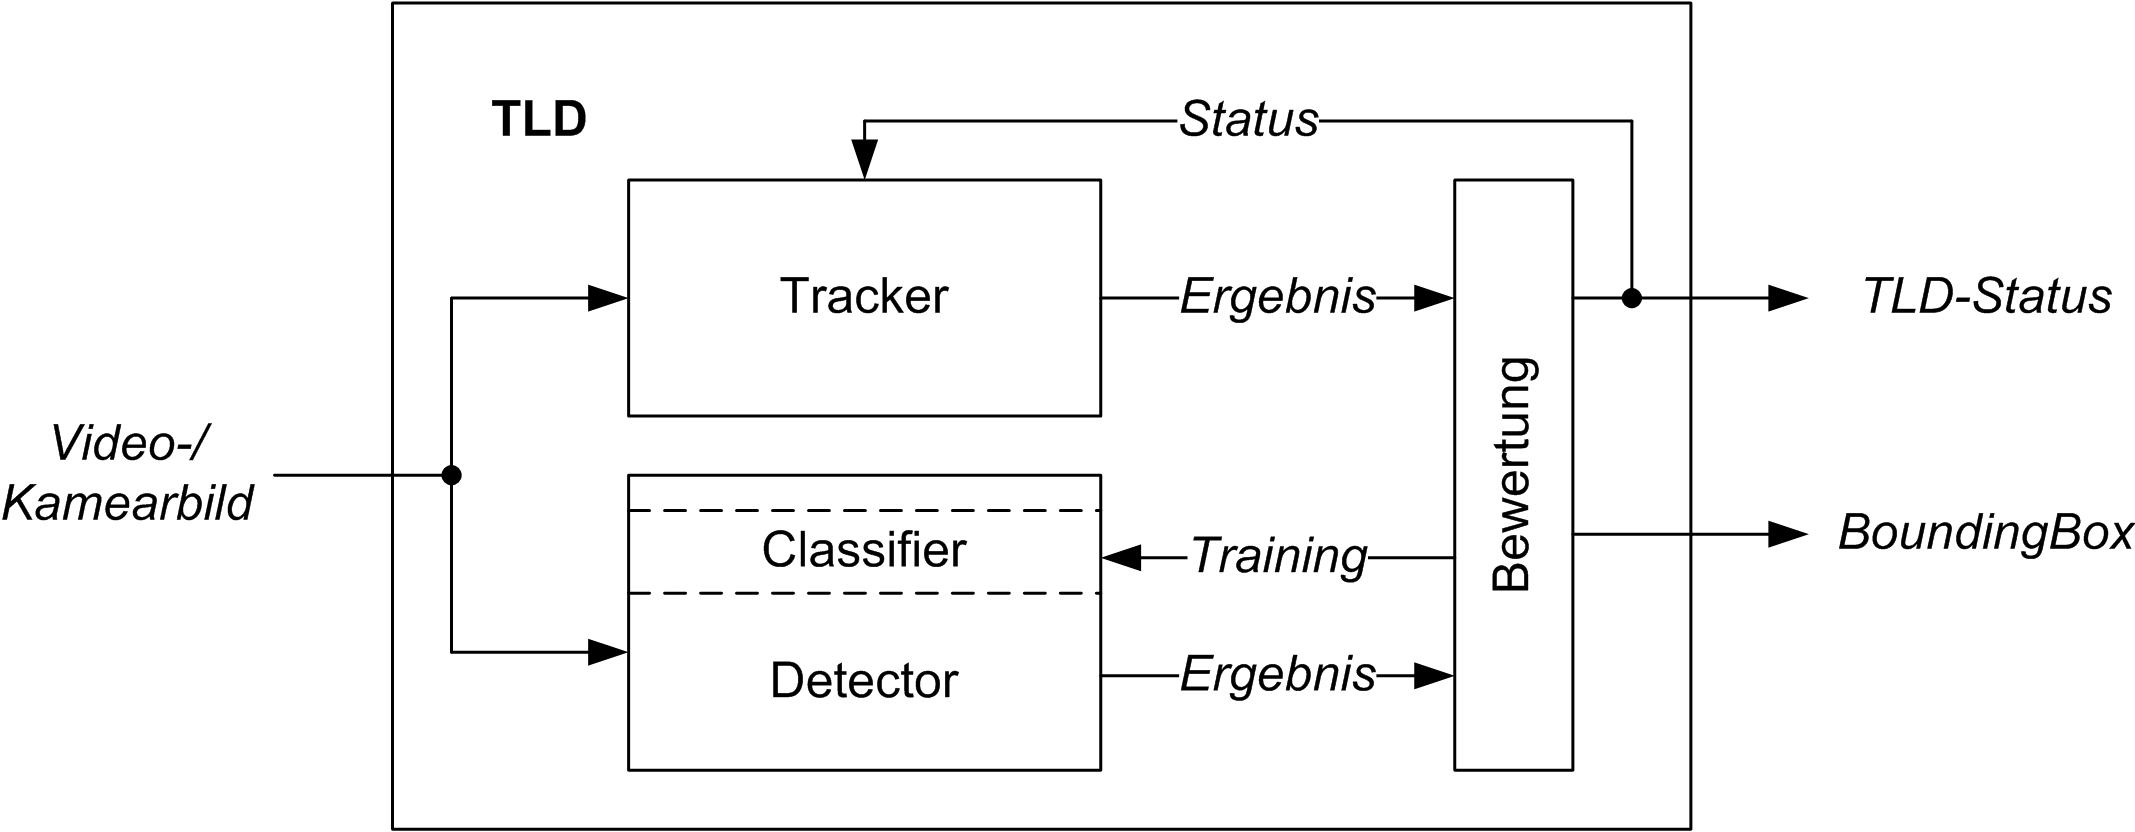
\includegraphics[scale=0.75]{../pictures/TLD-Framework.jpg}\caption{TLD-Schema}
\label{TLD-Schema}
\end{figure}

Als Sprache für die Umsetung wurde C++ gewählt, weil sie aufgrund der Möglichkeit relativ hardwarenah zu programmieren, schnelle Programme ermöglicht und durch OpenCV \cite{OCV} eine gut dokumentierte und umfangreiche Sammlung von Algorithmen speziell für den Bereich der Computer Vision liefert.

Im Anschluss zur Implementierung werden eine Reihe von Tests durchgeführt, die zu Beurteilung der Eignung von TLD für den speziellen Fall des Koptertrackings dienen. Es wird analysiert, welche Bedingungen zwingend gelten müssen, damit dieser Ansatz erfolgreich genutzt werden kann, und unter welchen Umständen sich TLD nicht eignet.


\subsection{Aufbau der Arbeit}
Die Arbeit ist wie folgt gegliedert.

\paragraph{Kapitel 1}
Das erste Kapitel stellt eine kurze Einführung in den Bereich der Computer Vision dar und leitet kurz den speziellen Bereich der Objekterkennung ein. Weiterhin wird die Zielsetzung der Arbeit definiert und der genutzte Algorithmus in Grundzügen vorgestellt.

\paragraph{Kapitel 2}
Dieses Kapitel gibt einen kurzen Überblick zu verwandten Arbeiten und verschiedenen Ansätzen zur Lösung des Problems des machinellen Sehens. Unterschiedliche Paradigmen und deren Einsatzgebiete werden kurz vergleichend vorgestellt.

\paragraph{Kapitel 3 }
Hier erfolgt die genaue Beschreibung von TLD. Es werden ausführlich die theoretischen und mathematischen Hintergründe erläutert und der Algorithmus im Detail vorgestellt.

\paragraph{Kapitel 4}
Im vierten Kapitel wir kurz die C++-Implementierung beschrieben. Zusätzlich werden die verwendeten Testszenarien vorgestellt und die durchgeführten Tests beschrieben.

\paragraph{Kapitel 5}
Den Abschluss dieser Arbeit bildet dieses Kapitel der Auswertung und Analyse er Testergebnisse sowie eine Reihe von Vorschlägen für etwaige Verbesserungen.

\paragraph{Anhang}
Im Anhang werden kurz OpenCV und OpenTLD vorgestellt, die zur Vervollständigung der Arbeit beigetragen haben. % Einleitung
		\cleardoublepage % -*- root: diplomarbeit.tex -*-
\section {Verwandte Themen }
Arbeiten, die sich speziell mit dem Tracken von Quadro- oder Hexakopter beschäftigen, gibt es derzeit kaum. Im folgenden Abschnitt werden deshalb prinzipielle Tracking und Detection-Ansätze sowie verschiedene Machine Learning-Methoden vorgestellt. Ein strikte Trennung von Tracking und Detection ist im Übrigen kaum möglich, das aktuelle Algorithmen meist eine Kombination darstellen. Prinzipiell ist in jedem Ansatz auch eine Objektrepräsentation vorhanden, die mittels maschinellem Lernen online beziehnungsweise offline vorbereitet und gelernt werden muss.

\subsection{Object Tracking}
Object-Tracking ist, allgemein gesprochen, das Verfolgen von bewegten Objekten in einer Bildsequenz über die Zeit mittels Bewegungsschätzung. Dabei ist die Anzahl der gerade in den letzten Jahren entwickelt Ansätze hoch und variantenreich. Sie unterscheiden sich zum einen in der Repräsentaiton des Objekts, mittels Konturen, Punkte, Modelle oder optischem Fluss, als auch in der Schätzmethode. Ein verbreiteter und auch in TLD genutzter Ansatz ist das Frame-to-Frame Tracking, bei dem die Position des Objekts im Bild aufgrund der Daten des Vorgängerbildes geschätzt wird.

Beim Template-Tracking \cite{OPT}\cite{GFT}\cite{KBT} wird ein Objekt als Template (Histogramm oder Patch) erfasst und die Bewegung (Motion) ist als Änderung mit dem kleinesten Missmatch zum Kandidaten für das gesuchte Template definiert. Je nach Realisierung ist das Template statisch\cite{KBT} oder flexibel \cite{OPT}\cite{GFT}, es kann sich also während des Trackens ändern. Es gibt auch Ansätze, die eine Mischung aus beidem implementieren \cite{TUP}\cite{SMAT}\cite{RDT} oder auch nur Teile des Templates nutzen \cite{ROAM}\cite{RFT}.

Um dem Nachteil der eingeschränkten Modellierung durch Templates zu begegnen, wurden weitere Repräsentationen für die Objekte entwickelt, beispielsweise die generative Modellierung. Die Idee hierbei ist, das Objekt mittels Parameter und Abhängigkeiten zu beschreiben. Diese Modelle werden entweder offline \cite{ETR} oder online während des Trackens erzeugt \cite{RFT}\cite{VTD}. Allerdings birgt das auch Nachteile, wie zum Beispiel bei detailreichen Hintergründen. Hier kann ein solcher Tracker leicht fehlschlagen. Deshalb wird neben dem Objekt auch die Umgebung modelliert, zum Beispiel als negative Klasse, wobei das Objekt selbst dann die positive Klasse bildet. Hierbei sind vor allem lernfähige Tracker von Bedeutung, da sie, im Gegensatz zu ihren statischen Pendants, während der Abarbeitung das Wissen über das Objekt und seine Umgebung sammeln, wodurch eine erhöhte Flexibilität erreicht wird. Dies geschieht mittels Erzeugnung von Klassifier \cite{ONS}\cite{ENT}\cite{OBT}. 

Neben der Modellierung lässt sich auch die Methodik spezifizieren. Hierbei wird von drei Grundformen ausgegangen: Point-Tracking, Kernel-Tracking und Silhouette-Tracking. Jede hat ihre spezifischen Eigenschaften und werden je nach unterschiedlichem Einsatz der späteren Applikation genutzt.

\subsubsection{Point-Tracking}
Allgemein gesrpochen wird das zu verfolgende Objekt durch Punkte repräsentiert, die von einem Bild $t-1$ im Folgebild $t$ gesucht werden. Dieses Verfahren weisen eine Reihe von Schwierigkeiten, wie das Handhaben von Verdeckungen oder falsche Punktdetektionen, auf. Unterschiedliche Ansätze und Strategien werden deshalb genutzt, um diesen Schwierigkeiten entgegenzuwirken und Lösungen zu finden. Diese Ideen können in \textit{deterministische} und \textit{statitische} Methoden eingeteilt werden. 

{\bf Deterministische Ansätze } definieren eine Kostenfunktion $f$ für jedes Objekt in $t-1$ und versuchen durch Minimierung dieser Kosten und einer Reihe Bedingungen (Constraints) das korrespondierende Objekt in $t$ zu finden. Constraints können hierbei sein:

\begin{itemize}
\item Das Objekt verändert sein Erscheinungsbild von einem Bild zum nächsten nicht oder nur sehr wenig \cite{FPIS}
\item Die maximale Geschwindigkeit, mit der sich ein Objekt bewegt, begrennzt den Radius, in dem das Objekt im Folgebild erscheinen kann.
\item Richtungs- und Geschwindigkeitsänderungen eines Objekts sind eher klein.
\item Objekte in der realen Welt sind starr, weshalb die verhältnismäßige Entfernung zweier Punkte sich nicht ändert.
\item $\dots$
\end{itemize}
Diese Bedingung sind nicht auf die deterministischen Methoden beschränkt, sondern finden auch in den statitischen Ansätzen Verwendung. 

{\bf Statistische Methoden} modellieren Zustandräume zu bestimmten Objekteigenschaften wie zum Beispiel Geschwindigkeit oder Position im Bild. Der Tracking-Verlauf wird dann als eine Sequenz von Zuständen $X^{t}:t=1,2,\dots$ aufgefasst, wobei, und das ist der Unterschied, das Bildrauschen $W^{t}:t=1,2,\dots$, das unweigerlich auftritt, in die Berechnung einfließt. So wird die Statusänderung über die Zeit für ein sich durch eine Sequenz von Bildern bewegendes Objekt beispielsweise durch die Formel $X^{t}=f^{t}(X^{t-1})+W^{t}$ berechnet. Um solche Zustandsräume für das Objekttracking, also für das Schätzen der Positionsänderung des Objekts von einem Bild zum Folgebild, gibt es wiederum verschiedene Ansätze, die hier jedoch nicht näher vorgestellt werden. Zu nennen sind in diesem Zusammenhang allerdings der \textit{Kalman}-Filter\cite{KAF} für lineare Systeme und der \textit{Particle}-Filter \cite{PAF} für nichtlineare Systeme, die mit großem Erfolg in Tracking-Algorithmen verwendet wurden.

\subsubsection{Kernel-Tracking}
Anders als beim Point Tracking dient hier eine Repräsentation des gesamten Objekts beziehungsweise einer Objektregion als Vorlage, und nicht nur einzelne Punkte. Auch hier unterscheiden sich einzelne Systeme und Ansätze hinsichtlich der Objektdarstellung, der Methodik und auch der Anzahl der zu verfolgenden Objekte. Zum Beispiel wird das Objekt mittels Template, oftmals bestimmte Color Features oder Histogramme, repräsentiert, das dann im aktuellen Bild gesucht wird. Die Postition wird dann mittels Ähnlichkeitsberechnung, beispielsweise durch Kreuzkorrelation, ermittelt. Am Ende wird die Region des Bildes als Objekt markiert, die dem Template am ähnlichsten ist. Der Nachteil dieses \textit{Template-Matching}-Verfahrens liegt vor allem in der rechenintensiven Methodik, da sie im Ansatz brute-force ist - es wird das gesamte Bild nach dem Template abgesucht. Dabei werden auch unterschiedliche Skalierungen, Orientierungen oder Transformationen des Templates gesucht, wodurch der eigentliche Berechnungsaufwand erzeugt wird. Verbesserungen in der Laufzeit können beispielsweise durch die Einschränkung des Suchraums oder die Arbeit mit integralen Bildern\cite{INT} erreicht werden.

Ein weiteres Verfahren, das auch in TLD Verwendung findet, ist das Tracken mittels \textit{optischem Fluss}, die es durch Lucas und Kanade\cite{OPT} vorgeschlagen und später durch Tomasi und Kanade\cite{LKT} erstmals zum Tracken implementiert wurde. Die Grundidee ist die Berechnung eines Vectorfeldes, unter Annahme konstanter Helligkeit, das für jeden Pixel im Bild die Bewegungsrichtung und -geschwindigkeit von einem Bild zum nächsten enthält. Für das Tracken wird nun ein ROI im Bild (das Objekt) ausgewählt. Dann werden aus dieser Region bestimmte Pixel für die Berechnung der Position des Objekts mittels des optischen Flusses im Folgebild herangezogen. Im Anschluss wird die Qualität der Berechnung mittels affiner Transformation zwischen dem gesuchten und dem gefundenen Patch evaluiert. Wenn die mittlere quadratische Abweichung aller Pixel zu hoch ist, wird das Ergebnis verworfen, ansonsten wird das Tracken forgesetzt.

Die genannten Verfahren eignen sich vor allem zum Single-Object-Tracking. Für das gleichzeitige Verfolgen von mehreren Objekten gibt es andere Kernel-Tracking-Algorithmen, die hier allerdings nicht näher vorgestellt werden.

\subsubsection{Silhouette-Tracking}
Nicht jedes Objekt, das getrackt werden soll, kann durch eine einfache geometrische Figur wie ein Rechteck oder ein Elypse repräsentiert werden. Deshalb wird mittels Silhoutte-Tracking versucht, solche komplexen Objekte anhand ihrer Kontour zu repräsentieren. Außerdem motiviert zu diesem Ansatz die Tatsache, dass auch der Mensch Objekte nur anhand ihrer Silhouette erkennen kann. Da in dieser Arbeit dieses Verfahren keine Rolle spielt, sei es nur zur Vollständigkeit erwähnt (ODER SOLLTE ICH DOCH NOCH MEHR DAZU SCHREIBEN?)

Welche Methode letzendlich genutzt wird, hängt von dem späteren Einsatzgebiet des Trackers ab.

Dabei gehen die meisten Tracking-Algorithmen z.B. von einer gleichförmigen Bewegung des Objekts aus, also ohne plötzliche Bewegungsänderung. Die Geschwindigkeit beziehungsweise die Beschleunigung bleiben konstant, wodurch vorherige Informationen über das Objekt, wie Position und Größe, für das Tracken genutzt werden können und somit das Problem vereinfachen \cite{OTS}.

Allerdings haben die meisten Tracker eins gemein: Sie versagen, wenn das Objekt kurzzeitig nicht mehr sichtbar ist, entweder wenn es den Bildbereich verlässt oder zu stark durch ein anderes Objekt verdeckt wird. Zusätzlich neigen sie meist zum Drift. Sie verlieren im Laufe der Abarbeitungszeit ihren Fokus und müssen dann reinitialisiert werden.

\subsection{Object Detection}
Object Detection ist das Finden eines Objekts in einem Bild beziehungsweise einer Bildsequenz. Grundlage bildet hier vor allem die Repräsentation des Objekts im Speicher und die damit verbundene Suchlogik. Im Laufe der letzten Jahre wurden auch hier unterschiedliche Repräsentationen entwickelt und untersucht \cite{OTS}:

\begin{description}
\item [{Punkte}] oder auch nur ein Punkt, der Centroid, repräsentieren das Objekt, was besonders für kleine Objekte in einem Bild nützlich ist.
\item [{Rechtecke}] oder Ellipsen, also zweidimensionale geometrische Figuren bilden das Objekt und bilden Grundlage vor allem für die Berechnung von Transformationen des gesuchten Objekts, um entsprechende Änderungen zu modellieren.
\item [{Silhouetten}] und Konturen bilden die Begrenzung des Objekts, und werden vor allem bei der Detektion von komplexen Objekten genutzt.
\item [{Patches}] des Objekts, die als Templates für die Suche dienen.
\item [{Multi-Shape-Patches}] bilden Teile eines zusammenhängenden Objekts. Die Verbindungen können durch unterschiedliche Verfahren, wie z.B. kinetic motion models, berechnet werden.
\end{description}

Alle genannten und ungenannte Repräsentationsverfahren können und werden in der Praxis und je nach Anwendungsgebiert kombiniert werden. Die große Herausforderung besteht nun vor allem im Segmentieren der gewählten Repräsentationen. Je nach Anwendungsfall ist eine solche Berechnung technisch leicht oder kompliziert zu realisieren. Einige Verfahren werden nun kurz vorgestellt.

\subsubsection{Point-Detectors}
bla

\subsubsection{Background Substraction}
bla

\subsubsection{Image Segmentation}
bla

\subsection{Maschinelles Lernen}
Seit Mitte der 1990er Jahren halten Methoden aus dem Bereich des Machine Learning Einzug in das Gebiet der Objekterkennung. Und heutzutage gibt keinen neuen Detection-Ansatz mehr, der ohnen einen gewissen Teil \textit{Intelligenz} auskommt, wie auch TLD. Im Folgenden wird daher ein kurzer Überblick über verschiedene Lern-Ansätze gegeben mit Verweisen auf Implementierungen in der Bildverarbeitung gegeben.

\subsubsection{Methoden}
Eine genaue Definition für Machinellen Lernen zu finden ist schwierig, da die Einsatzgebiete der verwendeten Methoden und Ansätze sehr vielfältig sind. Eine der erste und sicher treffensten ist die Definition von Arthur Samuel (1995):
\begin{quote}
Maschine Learning: Field of study that gives computers the ability to learn without being explicitly programmed. 
\end{quote}
Eine aktuelle und eher mathematische Formulierung findet Tom Mitchel (1998):
\begin{quote}
Well-posed Learning Problem: A computer program is sait to \textit{learn} from experience $E$ with respect to some task $T$ and some performance measure $P$, if its performance on $T$, as measured by $P$, improves with experience $E$.
\end{quote}
Im Falle der Objektdetektion ist ``Finde das Objekt'' die Aufgabe $T$, die zugrundeliegenden Beispiele, also die Daten, die das Objekt beschreiben, sind die Erfahrung $E$ und der Erfolg ``Objekt gefunden'' ist $P$.

Lernalgorithmen lassen sich in verschiedene Klassen enteilen:
\begin{itemize}
\item Superviced Learning, 
\item Unsupervised Learning,
\item Reinforcement Learning und
\item Recommender Systems,
\end{itemize}
wobei die ersten beiden Klassen im Bereich vermehrt im Bereich der Bildverarbeitung Verwendung finden.

Ohne im Detail Maschinelles Lernen vorzustellen, besteht jede Methode im Wesentlichen aus drei Komponenten: Das Training-Set, also das Model $M$ mit den $m$ Beispielen, das als Wissensbasis dient, der Lernalgorithmus (Kostenfunktion??), der als Eingabe $M$ erwartet, und der Bewertungsfuktion $h$, die für eine Eingabe $x$ eine Schätzung $y$ vornimmt. Die Funktion $h$ bestimmt hierbei die Abhängigkeit der Daten in $M$.

\paragraph{Supervised Learning}
Überwachtes Lernen. Man gibt Beispiele mit einem entsprechenden Ergebnis (Wert oder Klassefizierung) vor. Man sagt auch, dass die Beispiele gelabelt sind. Der Algorithmus kann dann anhand dieser gelernte Beispiele bestimmen, wie das neue Beispiel bewertet werden muss (also entweder wird ein Wert bestimmt oder eine Klassifzierung vorgenommen.

Hierbei unterscheidet man zwei Problemarten, die sich hinsichtlich der Berechnungsart und ihres Outputs unterscheiden:
\begin{enumerate}
\item Regression und 
\item Klassifikation.
\end{enumerate}
Regession wird verwendet, wenn zu einer bestimmten Eingabe ein konkreter (reeller) Wert erwartet wird. Klassifikation versucht hingegen die Eingabe einem diskreten Wert, also z.B. einer Klasse, zuzuordnen. Für Details wird an dieser Stelle auf die Fachliteratur verwiesen.

\paragraph{Unsuperviced Learning}
Hier versucht der Algorithmus für eine Anfangsmenge an Beispielen eigene Labels zu finden. Dazu werden sie anhand bestimmter Kriterien zu bestimmten Klassen zugeordnet (z.B. Entfernung). Ein Beispiel ist z.B. das Clustern von Daten.

\begin{comment}
	(Hier werden die prinzipiellen Arbeitsweisen des Core-Algorithmus TLD dargestellt und erläutert. Einleitend werden sie anhand von Diagrammen/Bildern/Beispielen erläutert, unter den folgenden Teilüberschriften wird vertiefend erklärt.

	Die Initialisierung des Algorithmus erfolgt über die Definition der BoundingBox. Dies kann auf unterschiedliche Weise, wie z.B. das Markieren eines Objekts in einem Kamera- oder Videobild, oder durch vorgeschaltete Programmteile, die auf das Erkennen eines bestimmten Objekts trainiert wurden, geschehen. Ausgehende von diesem ersten Bild werden die einzelnen Komponenten initialisiert. )
\end{comment}

\subsection{Beispiele für Tracking-Implementationen}
Das Feld der Objekterkennung ist weit und es gibt eine Vielzahl von unterschiedlichen Anwendungsszenarien. Im Folgenden wird eine kleine Auswahl solcher Szenarien vorgestellt, welche die oben genannten algorithmischen Ansätze implementieren.

\subsubsection{Gesichtserkennung}
durch Farbe, Bewegung, Kombination aus beiden (alles eher schlecht), Besser: Neuronal Netze, Modelbasiert und das allerbester: Weak Classifier von viola and jones,

\subsubsection{Fußgänger}
background seperation, foreground-silhuette-extraction kopf-detection, template-models

\subsubsection{Straßenschilder}
bla

\subsubsection{Schrift}
bla

\subsubsection{Autos}
bla % Verwandte Themen
		\cleardoublepage % -*- root: diplomarbeit.tex -*-
\section{Tracking Learning Detection - TLD}
	Die originale Implementation von TLD erfolgte in Matlab. Teil dieser Arbeit ist eine Adaption in C++. Zum Verständnis der einzelnen Komponenten und für die Darstellung der Arbeitsweise wird in diesem Kapitel der Algorithmus im Detail vorgestellt und theoretisch betrachtet.

	\subsection{Algorithmus}
	Die Gesamtheit des Algorithmus wird in {\em Algorithmus \ref{alg:TLD}} dargestellt. Die Initialisierung zu Beginn kann auf unterschiedlich Weisen erfolgen \ref{subsection:tld_init} und wird in dieser Darstellung nicht näher beschrieben. Es wird davon ausgegangen, dass als Eingabe eine BoundingBox $B_I$ definiert ist. Die zusätzlich benötigte Datenquelle ist eine Sequenz $Seq = \{I_1, I_2, \dots \}$ von Video- oder Kamerabilder. TLD verarbeitet dann nur ein Bild $J \in Seq$ zum Zeitpunkt $t$.

	\begin{algorithm}[H]
		\vspace{0.2cm}
		\KwData{$B_I, J$}
		\KwResult{$B_J$}
		\If{$B_I$ is not $NULL$} {
			$B_J^T \leftarrow track(I,J,B_I)$\;
		}
		$B_J^D \leftarrow detect(J)$\;
		$B_J \leftarrow compare(B_J^T,B_J^D)$\;
		\If{$isValid$ \& $doLearn $} {
			$train(J,B_J)$\;
		}
		$I \leftarrow J$\;
		\caption{Tracking-Learning-Detection}
		\label{alg:TLD}
		\vspace{0.2cm}
	\end{algorithm}
	Die Tracking-Komponente in Zeile 2 ist ein Frame-to-Frame Tracker (\ref{subsection:tracking}). Somit muss als Eingabe eine definierte BoundingBox übergeben werden. Ist diese jedoch nicht definiert, weil beispielsweise in der vorigen Iteration im Bild $I$ das gesuchte Objekt nicht gefunden werden konnte, wird der Tracker übergangen. Ist $B_I$ jedoch eine valide BoundingBox, wird zusätzlich $I$ übergeben und der Tracker schätzt im aktuellen Bild $J$ die Position des gesuchten Objekts. Das Ergebnis ist eine BoundingBox $B_J^T$.

	Der Detector in Zeile 4 wird vor dem ersten Aufruf von TLD initialisiert (\ref{subsection:tld_init}). Dadurch sind die Classifier und das Sliding-Window Grid verfügbar, die als Basis dienen. Wissen über den vorherigen ``Erfolg'' einer Detection in Form von $B_I$ ist nicht notwendig. Die Rückgabe des Detectors wird in einem Array von BoundingBoxes $B_J^D$ gespeichert.

	Im Anschluss werden die Ergebnisse beider Komponenten bewertet und die BoundingBox $B_J$ im aktuellen Bild $J$ wird, sofern vorhanden, gesetzt. Falls die Bewertung für $B_J^T$ am höchsten ist, wird eine Trainingsphase der Classifier initialisiert (\ref{subsection:machine_learning}), da $B_J^T$ eine unbekannte Repräsentation des gesuchten Objekts darstellt.

	Zum Abschluss wird das aktuelle Bild für die nächste Iteration und als Tracking-Datum in $I$ gespeichert. Die Verarbeitung von $B_J$, wie die Ausgabe, erfolgt außerhalb von TLD.

	\subsection{Tracking}
	\label{subsection:tracking}
	Die Tracker-Komponente hat im Wesentlichen die Aufgabe die Bewegung eines Objekts $o$ zu schätzen, wobei typischerweise die Annahme besteht, dass das Objekt in einer Bildsequenz sichtbar ist. Es gibt in der Praxis eine Reihe von Ansätzen, die sich hinsichtlich der Repräsentation des Objekts, zum Beispiel als Punkte, Kontouren, Modelle oder optischer Fluss, als auch der algorithmischen Verarbeitung unterscheiden.

	In dieser Arbeit wird, wie im grundlegenden TLD-Ansatz, der MediaFlow- Tracker \cite{MFT} implentiert. Der Grundgedanken basiert auf der\textit{ forward-backward consistency assumption}, die besagt, dass erfolgreiches Verfolgen unabhängig von der Richtung des Zeitflusses sein sollte. Als erstes wird eine Menge von gleichverteilten Punkten, definiert durch die BoundingBox, in einem Bild $t$ erzeugt. Im nächsten Schritt erfolgt die \textit{forward} Bestimmung des optischen Flusses mittels Lucas-Kanade-Algorithmus \cite{OPT} im Bild $t+1$. Die Punktemenge, die dadurch ermittelt wurde, wird nun \textit{backward} für die Bestimmung des optischen Flusses im Bild $t$ genutzt. Die Informationen aus beiden Lucas-Kanade-Berechnungen werden zur Bestimmung es \textit{Forward-Backward Errors (FB)} um fehlerhafte Punkte zu filtern. Die verbliebenen Punkte bestimmen die Transformation der BoundingBox. Abbildung \ref{fig:MFT} verdeutlicht das Prinzip.

	\begin{figure}
	\centering{}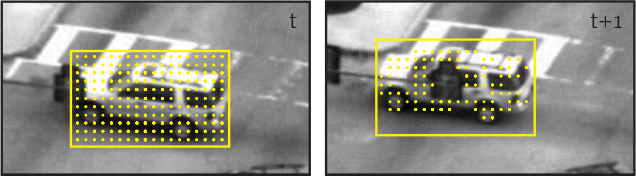
\includegraphics[scale=0.7]{../pictures/MediaFlow_0.png}\caption[Arbeitsweise des Median Flow Trackers]{Arbeitsprinzip des Median Flow Trackers. Alle Punkte, die sowohl in $t$ als auch in $t+1$ vorhanden sind, werden als Grundlage für die Berechnung der BoundingBox gentutzt. (Quelle: \cite{MFT})\label{fig:MFT} }
	\end{figure}

	\subsubsection{Der optischen Flusses und der Lucas-Kanade-Algorithmus}
	Die Berechnung des optischen Flusses entspricht im Wesentlichen der folgenden Aufgabe: Finde den Punkt $x$ aus Bild $I_{0}$ im Bild $I_{1}$ beziehnugsweise in einer Sequenz von Bildern $I_{1},..,I_{n}$. Lucas und Kanade gehen zur Berechnung von drei Annahmen aus.

	\begin{enumerate}
	\item \textit{Brightness constancy.} Das Erscheinungsbild eines Pixel eines Objekts in einer Sequenz bleibt unverändert. Für Grauwertbilder bedeutet das, dass die Helligkeit (\textit{brightness}) eines Pixels Konstant bleibt, wenn dieser von Bild zu Bild verfolgt wird.

	\begin{equation}
	I_{0}(x)=I_{1}(x+d)
	\end{equation}

	\item \textit{Temporal persistence. }Die Positionsänderung eines Objekts in einer Bildsequenz ist gering. Das bedeutet, dass die Geschwindigkeitsvectoren klein sind. Diese können im zweidimensionalen Fall mit der folgenden partiellen Ableitung berechnet werden:

	\begin{equation} I_{x}u+I_{y}v+I_{t}=0, \end{equation}
	mit $u,v$ als die gesuchten Geschwindigkeitsvectoren für die Koordinatenänderung für $x$ und $y$ im Bild $I$ und $I_{t}$ als zeitliche Änderung zwischen den Bildern. Allerdings ist diese Gleichung für einzelne Pixel nicht eindeutig lösbar, da durch die gesuchten Vectoren $u,v$ zwei Unbekannte existieren. Der Ergebnisraum wäre somit ein Linie und kein einzelner Punkt. Dieses Problem wird durch die dritte Annahme behandelt.

	\item \textit{Spatial coherence.} Punkte in einer Nachbarschaft gehören zur einer Oberfläche und verhalten sich gleich. Der gesuchte Punkt bildet das Zentrum eines $5\times5$ Pixel großen Ausschnitts.
	%\footnote{Auch andere Größen, wie $3\times3$ oder $7\times7$, sind denkbar. Allerdings wird die dritte Annahme mit steigender Ausschnittsgrößen nich mehr erfüllt%}.
	Mit Hilfe der Nachbarpunkte, deren Geschwindigkeit nach Annahme gleich ist, kann das folgende Gleichungssystem mit 25 Gleichungen erzeugt werden:

	\begin{equation}
	\left[\begin{array}{cc}
	I_{x}(p_{1}) & I_{y}(p_{1})\\
	I_{x}(p_{2}) & I_{y}(p_{2})\\
	\vdots & \vdots\\
	I_{x}(p_{25}) & I_{y}(p_{25})
	\end{array}\right]\left[\begin{array}{c}
	u\\
	v
	\end{array}\right]=-\left[\begin{array}{c}
	I_{t}(p_{1})\\
	I_{t}(p_{2})\\
	\vdots\\
	I_{t}(p_{25})
	\end{array}\right].
	\end{equation}
	\end{enumerate}
	Mittels Methode der kleines Quadrate kann die Lösung des Gleichungssystems minimiert werden. Für weitere Details zur Implementierung in \textit{OpenCV}
	siehe \cite{OCV}.

	\subsubsection{FB, NCC und Median Flow Tracker}
	Sei $S=(I_{t},I_{t+1},..,I_{t+k})$ eine Bildsequenz und sei $x_{t}$ ein Punkt zur Zeit $t$. Unter Verwendung eines beliebigen Trackers wird $x$ in $k$ Bildern aus $S$ verfolgt. Die erzeugte Trajektorie ist $T_{f}^{k}=(x_{t},x_{t+1},...,x_{t+k})$, mit $f$ für \textit{forward} der Länge $k$. Ziel ist es nun die Gültigkeit von $T_{f}^{k}$zu bestimmen. Hierzu wird der Punkt $x_{t+k}$\textit{backward} zum ersten Bild $I_{t}$ verfolgt. Der resultierende Trajektorie ist $T_{b}^{k}=(\hat{x}_{t},\hat{x}_{t+1},...,\hat{x}_{t+k})$, mit $b$ für \textit{backward} und $\hat{x}_{t+1}=x_{t+1}$. Der Fehler zwischen beiden Trajektorien ist definiert als $FB=distance(T_{f}^{k},T_{b}^{k})$, mit dem euklidischen Abstand zwischen dem initialen Punkt $x_{t}$ von $T_{f}^{k}$ und dem letzten Punkt $\hat{x}_{t}$ von $T_{b}^{k}$, also $distance(T_{f}^{k},T_{b}^{k})=||x_{t}-\hat{x}_{t}||$.

	Abbildung \ref{fig:Prinzip-des-Media} verdeutlicht das Erkennen von Tracking-Fehlern. Im linken Bild ist Punkt 1 in beiden Bildern sichtbar, also sind \textit{forward}- und \textit{backward}-Trajektorien identisch und der Tracker kann ihn korrekt verfolgen. Punkt 2 hingegen ist im rechten Bild verdeckt, was zu einer Bestimmung eines falschen Punktes führt. In der Konsequenz unterscheiden sich \textit{forward}- und \textit{backward}-Trajektorie und durch die Berechnung des \textit{Forward-Backward Errors} kann dieser Fehler leicht erkannt und behandelt werden.

	\begin{figure}
	\begin{centering}
	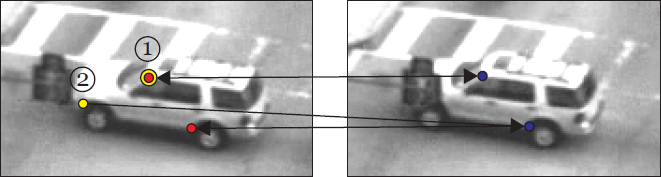
\includegraphics[scale=0.7]{../pictures/MediaFlow.png}
	\par\end{centering}

	\caption[Erkennen von Tracking-Fehlern]{Erkennen von Tracking-Fehlern. Die forward-backward-Trajektorien von Punkt 1 stimmen überein, da dieser in beiden Bildern existiert. Für Punkt 2 weichen sie jedoch segnifikant ab, weil dieser im zweiten Bild verdeckt ist. (Quelle: \cite{MFT})\label{fig:Prinzip-des-Media}}
	\end{figure}

	Neben dem Forward-Backward Error wird von Kalal et al.\cite{TLD}ein weiteres Messverfahren implementiert, der die Leistungsfähigkeit des Trackers signifikant verbessert\cite{MFT}. Mittel hierfür ist der \textit{Normalized Crorrelation Cefficient (NCC)}. % \begin{comment} HIER NOCH DIE FORMEL??? \end{comment}
	Es werden nicht nur die gesuchten Pixel, sondern auch deren umgebeneNachbarn analysiert. Dazu werden $10\times10$ Pixel große Patches, ausgehend vom verfolgten Punkt, generiert und mit einem ebenso erzeugten Patch des möglicherweise entsprechenden Punktes auf Ähnlichkeit untersucht. Sind sich beide ähnlich genug, dann wird der gefundene Punkt als valide angesehen.

	Der implentierte \textit{Median Flow Tracker} wendet das \textit{Forward-BackwardError}-Prinzip in Verbindung mit der Berechnung des \textit{NCC} entsprechend \cite{key-5} an. In Alg.\ref{alg:tracking} ist der Algorithmus skizziert. Als Eingabe dienen das letzte Bild $I$ mit der dazugehörige BoundingBox$B_{I}$ sowie das Folgebild $J$. Zur Berechnung der gültigen Punkte werden die Mediane des FB $median_{fb}$und des \textit{NCC} $median_{ncc}$genutzt. Hierbei werden die Punkte verworfen, deren FB größer als $median_{fb}$ und deren Ähnlichkeitswert kleiner als $median_{ncc}$ ist. Falls $median_{fb}$ größer als ein Treshold $th_{fb}$ ist, wird das Ergebnis durch LK als falsch interprätiert und verworfen. Die restlichen Punkte und $B_{I}$ dienen zur Berechnug der nächsten BoundingBox $B_{J}$. Hierzu wird der Median der Abstände aller Punkte in $I$ und in $J$ berechnet die Änderungen als Grundlage für die Verschiebnung in x- und y-Richtung genutzt. Die Skalierung von $B_{J}$ ist die relative
	Änderung der Abstände.

	\begin{algorithm}[H]
	\vspace{0.2cm}
	\KwData{$I,J,B_{I}$}
	\KwResult{$B_{J}^T$}
	Generiere Punkte $P = p_{1},\ldots,p_{n}$ mittels $B_{I}$\;
	\For{ $p_{i} \in P$ } {
		$p'_{i} \leftarrow LK(p_{i})$\;
		$p''_{i} \leftarrow LK(p'_{i})$\;
		$fb_{i} \leftarrow |p_{i}-p''_{i}|$\;
		$ncc_{i} \leftarrow NCC(p_{i},p'_{i})$\;
	}
	$median_{fb}\leftarrow median(fb_{1}\ldots fb_{n})$\;
	\eIf{$median_{fb}>th{}_{fb}$} {
		$B_{J}^T \leftarrow \emptyset$\;
	} {
		$median_{ncc} \leftarrow median(ncc_{1}\dots ncc_{n})$\;
		$q \leftarrow validePoints(p,median_{fb},median_{ncc})$\;
		$B_{J}^T \leftarrow calcBoundingBox(q,B_{I})$\;
	}
	\caption{Tracking}
	\label{alg:tracking}
	\vspace{0.2cm}
	\end{algorithm}

	\subsection{Detection}
	\label{subsection:detection}
	Wenn das verfolgte Objekt den Bildbereich verlässt oder durch andere Objekte verborgen wird, kann die Tracker-Komponente nicht weiterarbeiten. Das Model zur Berechnung der Trajektorie fehlt. Aus diesem Grund ist eine Detection-Komponente erforderlich, die versucht das Objekt im Bild zu finden. Typischerweise ist diese Aufgabe recht aufwendig und die Umsetzung stark von der Art der Repräsentation des Ojekt-Modells abhängig.

	In dieser Arbeit wird wie in \cite{TLD} beschrieben, ein kaskadierender Detector implementiert. Grundlage für das Durchsuchen eines Bildes ist die \textit{Sliding-Window}-Methode \cite{key-6}. Hierbei wird ein Gitter definiert, das über das Bild gelegt wird. Jedes Feld des Gitters ist ein Ausschnitt (\textit{window}) des Bildes und wird einzeln durch mehrere Klassifizierer bewertet. Sollte ein solches Teilbild am Ende der Kaskade nicht verworfen worden sein, ist es ein Kandidat für das gesuchte Objekt. Die Größe des Gitters wird durchdie initiale BoundingBox bestimmt, da die einzelnen Felder Skalierungen dieser sind.

	Die Kaskade des Detectors besteht aus drei Teilen, dem Varianzfilter, dem \textit{Ensemble-Classifier} und als letzte Instanz der \textit{NearestNeigbour-Classifier}, die im folgenden einzeln vorgestellt werden. Dabei ist der Grundgedanke, dass ein gesuchtes Objekt komplexer als der Bildhintergrund ist. Jeder Teil hat die Aufgabe, die \textit{windows} zu Klassifizieren und entweder zu verwerfen, da sie nicht dem gesuchten Objekt entsprechen können, oder an den nächsten Klassifizierer weiterzureichen, wenn keine eindeutig negative Aussage getroffen werden kann. Nach einer kompletten Abarbeitung des Gitters werden die übrig gebliebenen Kandidaten mittels Cluster-Verfahren gruppiert. Als Kriterium dient der Grad der Überlappung der einzelnen \textit{windows.} Aus jedem Cluster wird abschließend eine gemittelte BoundingBox berechnet, die ein mögliches gefundenes Objekt repräsentiert. Im Gegensatz zu vielen anderen Detector-Ansätzen, benötigen diese Implementation keine offline-Trainingsdaten. Die Lernkomponente, bestehend aus Ensemble-Classifier und Nearest-Neighbour-Classifier, wird mit der ersten BoundingBox initialisiert. Alle weiteren Trainingsbeispiele werden mit Hilfe des Trackers und der P-N Learning-Komponente erzeugt. Genaueres folgt im Punkt Maschinelles Lernen.

	\begin{algorithm}
	\vspace{0.2cm}
	\KwData{$I$}
	\KwResult{$B_J^D$}
	$result = \{\}$\;
	\For{$g \in G$}{
		\If{$VarianceClassifier(I, g) == true$}{
			\If{$EnsembleClassifier(I, g) == true$}{
				\If{$NearestNeighbourClassifier(I, g ) == true$}{
					$result \leftarrow result + g$\;
				}
			}
		}
	}
	\If{$result.size > 0$}{
			$B_J^D \leftarrow cluster(result)$\;
	}
	\caption{Detection}
	\label{alg:detection}
	\vspace{0.2cm}
	\end{algorithm}

	\subsubsection{Objekt-Modell}
	Die Modellierung des Objekts und dessen Umgebung erfolgt in einer speziellen Datenstruktur
	\begin{equation}
	M=\{p_{1}^{+},p_{2}^{+},\dots,p_{m}^{+},p_{1}^{-},p_{2}^{-},\dots,p_{n}^{-}\}.
	\end{equation}
	Die Patches $p^{+}$bilden hierbei die positiven Beispiele, die das Objekt identifizieren ($p_{1}^{+}$bildet hierbei das initiale Objekt, das durch die Definition der BoundingBox erzeugt wurde). Die $p^{-}$ sind eine Sammlung negativer Beispiele, die aus der Umgebung der BoundingBox ermittelt werden. Während der Ausführung des Algorithmus' wird das Objekt-Modell stetig mit neuen positiven und negativen Beispielen erweitert. Die Strategie wird im Kapitel Maschinelles Lernen näher beschrieben.

	\subsubsection{Sliding-Window}
	Aus der initialen \textit{BoundingBox} werden alle möglichen Skalierungen und Verschiebungen dieser Box generiert. Damit wird das gesamte Bild mit den verschiedenen Größen und Positionen, die das Objekt annehmen kann, überdeckt. Für die Erzeugung des so entstehenden Gitters werden die folgenden Parameter genutzt: Skalierungs-Schritt$=1.2$, horizontale Verschiebung $=10\%$ der Breite, vertikale Verschiebung $=10\%$ der Höhe, Mindestgröße einer Box $=20\times20$ Pixel. Für ein Bild mit einer Auflösung von $640\times480$ Pixel ergeben sich bis zu $200.000$ \textit{BoundingBoxes}. Die tatsächliche Anzahl ist allerdings von der initialen BoundingBox abhängig. Für Geschwindigkeitsverbesserungen, kann die Mindestgröße einer Box auf $40\times40$ Pixel erhöht werden, wodurch nur noch bis zu $50.000$ BoundingBoxes erzeugt werden. Die Resultate des Detectors werden dadurch nicht signifikant schlechter.

	\subsubsection{Varianzfilter}
	Die erste Stufe des kaskadierenden Classifier bildet der Varianzfilter. Dieser vergleicht alle Patches, die durch das Grid gegeben sind, und verwirft die, deren Varianz kleiner als die Varianz des gesuchten Objekts ist. Dadurch können uniforme Regionen wie Hintergründe (Himmel, Wände etc.) schnell erkannt und verworfen werden um so den Suchraum zu verkleinern.

	Die Berechnung der Varianz kann sehr schnell mittels integralen Bildern (\textit{integral images}) erfolgen \cite{key-6}. Dabei handelt es sich um eine spezielle Datenstruktur, die eine einfache und schnelle Summierung von Pixelwerten beliebiger Regionen in einem Bild in $O(1)$ erlaubt. Zur Veranschaulichung siehe Abb. \ref{integralImg}. Für eine Bild $i$ der Größe $w,h$ ist das integrale Bild $ii$ eine Struktur der Größe $w+1,h+1$, wobei die erste Zeile und die erste Spalte jeweils mit $0$ gefüllt sind. Alle anderen Pixelwerte entsprechen der Summe der Pixel links und über dem Pixel, addiert mit dem eigenen Wert.

	\begin{figure}[h]
	\centering{}%
	\begin{tabular}{|c|c|c|}
	\hline
	4 & 3 & 1
	\tabularnewline
	\hline
	\hline
	2 & 4 & 3
	\tabularnewline
	\hline
	8 & 10 & 4
	\tabularnewline
	\hline
	\end{tabular} %
	\begin{tabular}{|c|c|c|c|}
	\hline
	0 & 0 & 0 & 0
	\tabularnewline
	\hline
	\hline
	0 & 4 & 7 & 8\tabularnewline
	\hline
	0 & 6 & 19 & 30
	\tabularnewline
	\hline
	0 & 14 & 43 & 57
	\tabularnewline
	\hline
	\end{tabular}\caption{Darstellung der Pixelwerte eines $3\times3$ Bildes (links) und des
	dazugehörigen integralen $4\times4$ Bildes (rechts).}
	\label{integralImg}
	\end{figure}

	Die Berechnung kann in linearer Zeit mittels einmaliger Iteration über das Bild durchgeführt werden.

	$$ ii(x,y)=\underset{x'\leq x}{\sum}\underset{y'\leq y}{\sum}i(x',y'). $$
	Der Vorteil der integralen Bilder liegt nun in der schnelle Berechnung von Pixelwerten innherhalb rechteckiger Teilbildern, die dann für weitere Berechnungen oder als Vergleichskriterium dienen. Die Summe der Pixel für ein Quadrat $ABCD$, siehe Abb. \ref{Subwindow}, kann mit Hilfe von vier Array-Referenzen berechnet werden. Da $D$ die Summe aller verherigen Pixel ist, müssen die Werte von $B$ und $C$ subtrahiert werden, weil sie nicht Teil von $ABCD$ sind. Da allerdings der Wert von $A$ dadurch zweimal abgezogen wurde, muss $A$ abschließend wieder dazuaddiert werden. Daraus ergibt sich die Formel $$ABCD=D+A-C-B$$ für die Summe der Pixelwerte eines Teilbildes $ABCD$.

	\begin{figure}
	\centering{}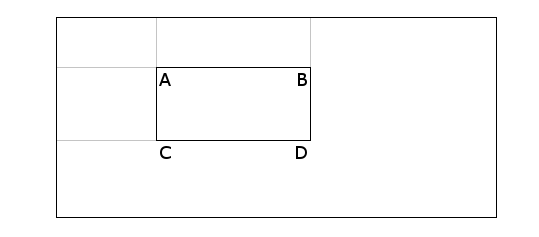
\includegraphics[scale=0.7]{../pictures/IntegralImage.png}\caption{Teilbild $ABCD$}
	\label{Subwindow}
	\end{figure}

	Neben dem integralen Bild können auch weitere Strukturen, wie das quadratische integrale Bild $ii^{2}$ auf ähnliche Weise berechnet werden. In der Implementierung wird das auch getan, um die Varianz durch $var(p)=ii^{2}(p)-i(p)^{2}$ zu berechnen. WELCHE VORTEILE HAT DAS GENAU??? HIER MUSS NOCH WAS ZUR ERKLÄRUNG HIN!!!

	Auf die beschriebene Weise werden nun die Varianzen der einzelnen möglichen Objekte, die durch das Grid definiert sind, mit dem Varianzwert des aktuellen BoundingBox verglichen, und bei einem geringeren Wert verworfen. Alle übrig gebliebenen Boxen werden im folgendenen \textit{Essemble Classifier} verarbeitet.

	\subsubsection{Ensemble-Classifier}
	Wurde ein Patch nicht durch den Varianzfilter verworfen, gelangt er zur zweiten Stufe der Kaskade, dem EnsembleClassifier. Dieser besteht aus einer Menge so genannter Base-Classifier, die einzeln eine Bewertung zu dem übergebenen Patch abgeben. Aus deren Ergebnisse wird ein Mittelwert gebildet, der dann die Bewertung des \textit{Ensemble-Classifiers} ist.

	\paragraph{Random Ferns}
	Grundlage des Klassifizierers ist die in XXX vorgestellte \textit{random fern classification}-Methode. Das Ensemble der Base-Classifier besteht aus $n$ Ferns, von denen jeder unabhängig den Patch $I$ bewertet. Dafür vollzieht jeder Fern $i$ eine Anzahl binärer Pixelvergleiche zweier zufällig gewählter Pixel im Patch, mit

	\begin{equation}
	f_{i}=\begin{cases}
	0, & I(d_{i,1})<I(d_{i,2})\\
	1, & sonst
	\end{cases}
	\end{equation}

	Aus den Vergleichen der einzelnen Features, also zweier Pixelwerte, wird ein binären Code $x$ erzeugt. Der entsprechende dezimale Wert ist wiederum Index für ein Feld von A-Posteriori-Wahrscheinlichkeiten $P_{i}(y|x)$, mit $y\in{0,1}$. Aus allen berechneten Wahrscheinlichkeiten jedes Ferns wird dann ein Mittelwert berechnet und falls diese kleiner als $0.5$ ist, wird der Patch verworfen.

	Die zufällig gewählten Features werden bei der Initialisierung des \textit{Ensemble-Classifiers} berechnet und bestehen während der Laufzeit des Programms unverändert. Da der Vergleich zweier Pixel ein sehr schwaches Unterscheidungskriterium ist, muss eine große Anzahl von Features für jeden Fern erzeugt werden. Anders ausgedrückt sollte das Feld der A-Posteriori-Wahrscheinlichkeiten möglichst viele Einträge haben. Für ein $P_{i}$ ergibt sich $2^{d}$ als Feldgröße, wobei $d$ die Anzahl der Features für ein $i$ist. In der Implementierung führt jeder Fern $13$ Pixelvergleiche durch, was in $8.192$ möglichen Codes resultiert. Die A-Posteriori-Wahrscheinlichkeit wird durch $P_{i}(y|x)=\frac{\#p}{\#p+\#n}$ berechnet, mit $\#p$ als Anzahl der positiven und $\#n$ als Anzahl der negativen Bewertungen eines Ferns $i$ für den Code $x$ ist.

	\begin{figure}[H]
	\begin{centering}
	\includegraphics[scale=0.5]{../pictures/EnsembleBeispiel.jpg}
	\par\end{centering}
	\caption{Prinzipielle Arbeitsweise der \textit{Base-Classifier}.}
	\label{EnCl}
	\end{figure}

	Abbildung \ref{EnCl} verdeutlich das Prinzip. Das Ensemble besteht aus drei Ferns mit jeweils vier Feature. Die in jedem Kästchen dargestellte Punkte stellen die Pixel im Bild da und werden jeweils paarweise verglichen. Pro Kästchen also der Pixelwert des schwarzer mit dem des weißen Punktes. Die vier binären Vergleiche pro Fern resultiert in einem binären Code, für Fern 1 ist dieser beispielsweise $1100$. Dieser Code wird nun dezimal interprätiert und dient als Index im\textit{ Posterior}-Array, im genannten Beispiel also $1100_{2}=12_{10}$ und damit $P_{1}[12]=0.6$.

	% \begin{comment}
	% ERKLÄRUNG ZUR FUNKTIONSWEISE DES FERNCLASSIFIER (Was sind Ferns? Die
	% Idee? Binäre KLassifizierung eines Bildes mittels ``Maske'' - da
	% sehr schwach muss es viele Klassifizierer geben (Das ist auch besser,
	% siehe Quelle {[}bla{]}), Ähnlichkeiten zu RandomForest, warum ist
	% Fern besser, Wie wurde implementiert, Initialisierung, Update etc...

	% Initialisierung: 10 pos (die besten, also conf > 0.5) und 100 neg
	% Beispiele (willkürlich)

	% Anfangs werden die Patches mit einem Gaußfilter (Standardabweichung von 3 Pixel)
	% \end{comment}
	\subsubsection{Template-Matching und Nearest-Neighbour-Classifier}

	Die vorherigen Stufen der Kaskade dienten vor allem zur Aussortierung falscher Kandidaten und damit die Verkleinerung des Suchraums. Das im Folgenden beschriebene Verfahren ist ein direkter Vergleich zwischen Patches und gespeicherten Repräsentationen von Bildern und damit die eigentliche Detektion.

	\paragraph{Template-Matching}
	Die letzte Stufe des Klassifizierers ist ein Nearest-Neighbour-Classifier, der mittels Template-Matching die verbliebenen Patches klassifiziert. Bei diesem Verfahren wird der gesuchte Patch (das Template) $T$ direkt in einem Bild $I$ gesucht, indem es über dieses geschoben und mittels einer Matching-Methode, in dieser Implementation durch Berechnung des (normalisierten) Korrelations-Koeffizienten, verglichen wird. Dabei wird der relative Mittelwert von $T$ mit dem relativen Mittelwert von $I$ verglichen. Das Ergebnis ist ein Wert zwischen $1$(perfekter Match) und $-1$(perfekter Missmatch). $0$ bedeutet, dass zwischen $T$ und $I$ keine Korrelation exisitert. Da es sich hierbei um eine sehr konservative und rechenintensive Vergleichsmethode handelt, bildet sie den Abschluss der Kaskade.

	Der Korrelations-Koeffizient wird wie folgt berechnet:

	\begin{equation}
	CC(x,y)=\underset{x',y'}{\sum}[T'(x',y')\times I'(x+x',y+y')]^{2}
	\end{equation}


	\begin{equation}
	T'(x',y')=T(x',y')-\frac{1}{(w\times h)\underset{x'',y''}{\sum}T(x'',y'')}
	\end{equation}


	\begin{equation}
	I'(x+x',y+y')=I(x+x',y+y')-\frac{1}{(w\times h)\underset{x'',y''}{\sum}I(x+x'',y+y'')}
	\end{equation}

	Um Fehler zu reduzieren, die durch eine unterschiedliche Beleutung des Templates $T$ und des Bildes $I$ entstehen können und damit	das Ergebnis verfälschen, wir der Koeffizient normalisiert. Zusätzlich wird das Ergebnis umgerechnet, so dass es im Intervall $[0..1]$	liegt.

	\begin{equation}
	S(x,y)=0.5(NCC(x,y)+1)
	\end{equation}

	\begin{equation}
	NCC(x,y)=\sqrt{\underset{x',y'}{\sum}T(x'y')^{2}\times\underset{x',y'}{\sum}I(x+x',y+y')^{2}}.
	\end{equation}

	\paragraph{Nearest-Neighbour-Classifier}
	Positive und negative Beispiele, die dem Klassifizierer für den Vergleich dienen, sind genormte $15\times15$ Pixel große Patches und werden	durch das Objekt-Modell $M$ repräsentiert. Der zu überprüfende Patch wird mit allen positiven und negativen Beispielen verglichen und es wird jeweils der größte Korrelations-Koeffizient berechnet. Diese dienen wiederum als Grundlage für die Ähnlichkeitsberechnung des Patches zur positiven Klasse. Es wird hierbei die relative Ähnlichkeit $S^{r}(p,M)=\frac{S^{+}}{S^{+}+S^{-}}$	berechnet und mit einem Threshold-Wert $\Theta$ verglichen, mit $\Theta=0.65$	\footnote{Werte für $\Theta$ zwischen $0.5-0.7$ sind ebenfalls zulässig und	bringen ähnliche Resultate \cite{TLD}. }. Gilt $S^{r}(p,M)>\Theta$, wird der Patch als positiv klassifiziert.

	Alle Patches, die zu diesem Zeitpunkt nicht durch die Kaskade verworfen wurden, bilden die Ausgabe der Detektor-Komponente. Typischerweise sind es mehrere Patches, die sich sehr ähneln und stark überlappen, und im Allgemeinen Teile des gesuchten Objekts repräsentieren. Das ist $\Theta$ geschuldet, denn die Patches werden nicht mit einem klaren Label für ``ist Objekt/ist kein Objekt'' versehen. Aus diesem Grund werden mittels Cluster-Verfahren Gruppierungen gebildet, aus denen abschließend die BoundingBox für das mögliche Objekt generiert wird.


	\subsubsection{Cluster-Verfahren}
	Nachdem der Detector eine Reihe von Patchen klassifiziert und mit	$p^{+}$ gelabelt hat, ergibt sich ein Problem. Im Idealfall sollten	alle Patches, die postitiv sind, also als Objekt erkannt wurden, mit $1$ und alle anderen mit $0$ bewertet werden \cite{BAB}. Dies ist in diesem Verfahren jedoch nicht möglich, da die Bewertung des Nearest-Neighbours	Werte zwischen $[\Theta..1]$ generiert und eine eindeutige Klassifizierung nicht möglich ist. Wegen des Sliding-Window-Ansatzes wird der Detector	fast immer Kandidaten finden, die sich sehr nahe an der eigentlichen Detektion befinden, siehe Abbildung \ref{abb:cluster}.

	\begin{figure}
		\begin{centering}
			% 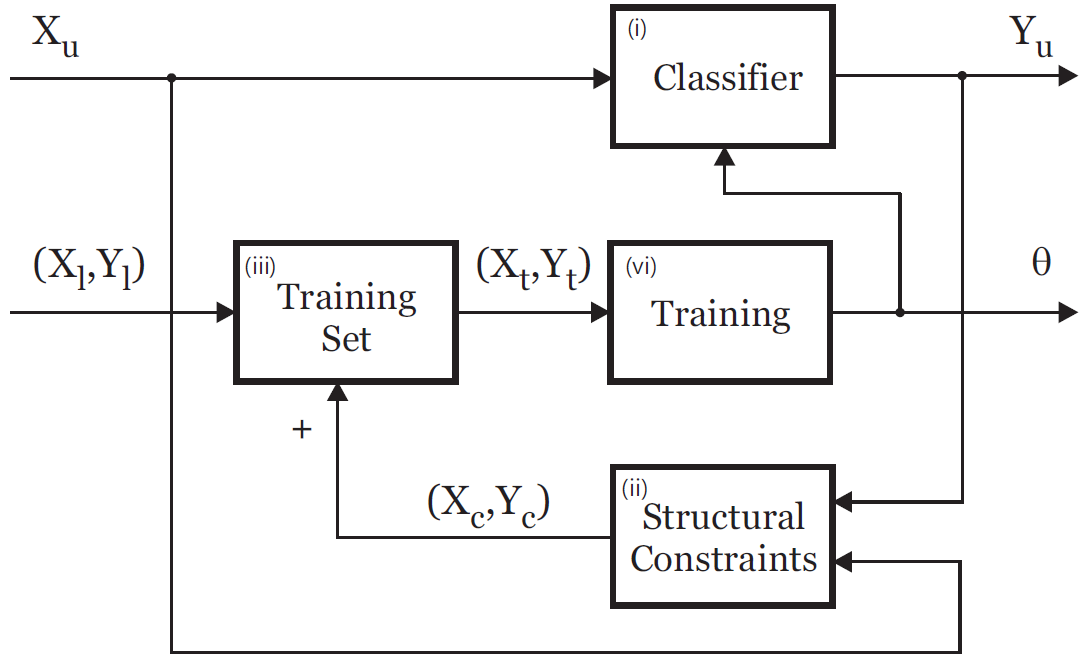
\includegraphics[scale=0.4]{../pictures/PN_LEARNING.png}
			ABBILDUNG! ÜBERLAPPENDE WINDOWS
			\caption{Clustering}
			\label{abb:cluster}
			\par
		\end{centering}
	\end{figure}

	Das heißt, dass im Normalfall ein einzelnes Window keine Objektpräsentation darstellt und dass es mehrere Kandidaten gibt, die nach der Kaskade als potentiell positive Objekte identifiziert werden. Die Behandlung dieses Problems erfolgt durch einen Cluster-Algorithmus. Kandidaten gehören zu einem Cluster, wenn sie sich mehr als $60\%$ überlappen und beispielsweise auch komplett ineinander liegen. Zur anschließenden Berechnung werden die Positions- und Größenwerte über diese Kandidaten gemittelt. Auf diese Weise werden eine oder mehrere Objektrepräsentation in Form von BoundingBoxen $B_J^D = \{B_1^D, B_2D, \dots\}$ erzeugt. An dieser Stelle wird als Ergebnis allerdings nur eine BoundingBox erwartet, da das Objekt zur Zeit $t$ nur einmal vorkommen kann. Der Algorithmus wird in Algorithmus \ref{alg:cluster} skizziert.

	\subsection{Maschinelles Lernen}
	\label{subsection:machine_learning}
	Die Tracking- und die Detection-Komponenten arbeiten unabhängig von einander, weshalb deren Ergebnisse zusammengeführt und bewertet werden müssen. Dies geschieht durch P/N-Learning \cite{PNL}. Gleichzeitig bildet dieser Ansatz die Grundlage des Lernens und damit des Trainierens
	des Fern- und des NearestNeighbour-Classifiers.

	\begin{algorithm}
	\vspace{0.2cm}
	\KwData{$B_J, J$}
	% \KwResult{}
	initialization\;
	\While{not at end of this document}{
	read current\;
	\eIf{understand}{
		go to next section\;
		current section becomes this one\;
	}{
		go back to the beginning of current section\;
	}
	}
	\caption{P/N-Learning}
	\label{alg:learning}
	\vspace{0.2cm}
	\end{algorithm}

	Hintergrund des semi-supervised learning-Prozesses sind postive (P)	und negative (N) Restriktionen (Constraints) für das Markieren (labeling)	des unmarkierten Datensatzes. Im Gegensatz zu Ansätzen, wie in \cite{TCL} \cite{CLU}, in denen die Daten als Unabhängig angesehen sind, Bilden der unmarkierte Datensatz bei P/N-Learning eine zusammenhängende \textit{Struktur} genannt. Im Fall der Object Detection bilden alle möglichen Patches des Bildes diese Struktur und die ufgabe besteht darin jeden dieser Patches entweder als positiv, und somit dem Objekt, oder als negativ, und damit dem Hintergrund, zuzuordnen. Da ein Objekt in einer Videosequenz temporär nur an einem Ort sichtbar sein kann, werden die Patches in diesem Bereich eine ähnliche postiven Markierung erhalten, Patches, die weiter weg vom Objekt sind, eine negative.

	Abbildung \ref{abb:pnl} gibt einen Überblick der beteiligten Komponenten und deren Zusammenhang von P-N Learning. Im Klassifizierer (i) (im	TLD-Ansatz sind das Fern- und NearstNeigbour Classifier) werden die unbestimmten Daten aus $X_{u}$ gelabelt. (ii) bilden die Constraints zur Bewertung der gelabelten Patches, ändern gegenballs die Labels und erweitern die Trainingsmenge (iii), die wiederum für das Training (iv) des Klassifizierers genutzt wird. Die genaue Erläutering der Arbeitsweisen erfolgt im Anschluss.

	\begin{figure}
	\begin{centering}
	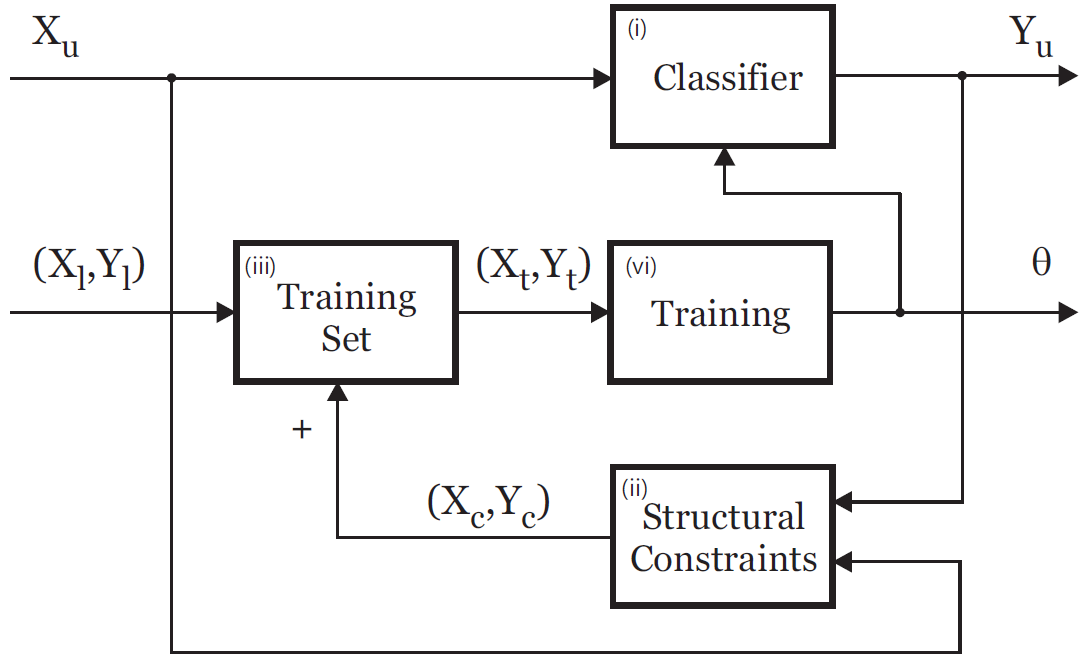
\includegraphics[scale=0.4]{../pictures/PN_LEARNING.png}\caption{Arbeitsweise P-N Learning (Quelle: \cite{PNL})}
	\label{abb:pnl}
	\par\end{centering}
	\end{figure}

	\subsubsection{P-N Learning}

	\begin{comment}
	Im Wesentlichen besteht jeder Lernalgorithmus aus zwei Funktionen: Bewertungsfunktion und Lernfunktion. Die Bewertung übernimmt hier der Classfifier. Lernen wird durch P-N wird durch Constraints vorbereitet - sie generieren die positiven und negativen Beispiele, wobei hier die positiven am Wichtigsten sind.
	\end{comment}

	Sei $X$ ein Beispielraum (Feature-Space) und $x\in X$ ein Beispiel, und sei $Y=\{-1,1\}$ ein Labelraum und $y\in Y$ ein Label. Eine Menge von Beispielen $X$ und mit entsprechenden Labels $Y$ sei die markierte (gelabelte) Menge $(X,Y)$. Die Aufgabe von P-N Learning ist die Funktion $f:X\rightarrow Y$, parametrisiert mit $\Theta$, von einer initialen Menge $(X_{l},Y_{l})$ zu lernen und mittels ungelabelter Daten $X_{u}$ dessen Arbeitsweise zu verbessern. . $f$ ist somit ein Classifier, der mittels bootstrapping trainiert wird.

	\paragraph{Bootstrapping}
	Lernen das Klassifizierers durch Erweiterung des Trainingsets mittels Beispielen, die durch die Constraints aus den ungelabelten Daten gewonnen werden. Initialisierung durch bereits gelabelte (also positive und negative Beispiele). Von da an erfolgt die Abarbeitung iterativ.

	In Schritt $k$ hat der Klassifizierer bereits $k-1$ mal Labels zu unmarkierten Beispielen bestimmt, mit $y_{u}^{k}=f(x_{y}|\Theta^{k-1})$, wobei in jedem Schritt nur ein Beispiel berechnet wird. Die Constraints bewerten im Anschluss die erzeugte Ausgabe und prüfen, ob die Labels den erwarteten Bedingungen genügen. Sollte dies nicht der Fall sein, werden sie gegenfalls umgelabelt und werden der Trainingsmenge hinzugefügt. Ist dieser Schritt abgeschlossen, wird der Klassifizierer mit Hilfe der erweiterten Trainingsdaten trainiert und die Abarbeitung beginnt mit der nächsten Iteration $k+1$ von vorn.

	\paragraph{Constraints}
	Die Constraints dienen zum Bewerten der Detection-Ergebnisse und zur Generierung der Trainingsmenge. Die wichtigste Aufgabe besteht darin, nur solche Beispiele für die Lernprozedur zu filtern, die ``gut genug'' und gleichzeitig ``nicht zu gut'' sind. Dazu wird das Ergebnis des Trackers mit der Ergebnismenge des Detectors verglichen. Hat der Detector ein Objekt gefunden, das mit dem des Trackers übereinstimmt, wird nicht gelernt, da die verwendete Datenbasis des Classifiers anscheinend gut genug war. Findet der Tracker allerdings ein Objekt, das nicht mit der Ergebnismenge übereinstimmt, wird geschätzt, welches Ergebnis am plausibelsten ist. Dies geschieht auf Grundlage der vorhanden Datenbasis.

	Hier können zwei Fälle eintreten:
	\begin{enumerate}
	\item Das Ergebnis des Trackers ist ``besser'': In diesem Fall ist die gefundene Version des Objekts noch nicht in der Datenbasis und dient als Grundlage für ein positives Beispiel in der nächsten Lernphase.
	\item Das Ergebnis des Detectors ist ``besser'': Damit wurde das gesuchte Objekt gefunden und der Tracker hat anscheinend aus unterschiedlichen Gründen den Fokus verloren. Deshalb muss er reinitialisiert werden, und zwar auf das Objekt, das der Detector gefunden hat.
	\end{enumerate}

	Ein Constraint ist in erster Linie eine Funktion, die als Parameter eine Menge von gelabelten Beispielen des Classifiers $(X_{u},Y_{u}^{k})$ erwartet und eine Menge von Beispielen $(X_{c}^{k},Y_{c}^{k})$, deren Label geändert wurden, als Ergebnis liefert. Die Anzahl dieser Constraints kann in diesem Fall beliebig sein, allerdings werden sie in zwei Kategorien geordnet: $P$ und $N$.

	\textit{P-constraints} dienen zur Identifikation von Beispielen, die vom Classifier zwar als negativ bewertet, von den Constraints allerdings als positiv angesehen werden. \textit{N-constraints} hingegen identifizieren negative Beispiele, die vom Classifier fälschlicherweise als postitiv bewerten wurden. Dabei sind in der $k$-ten Itereration $n^{+}(k)$ die Anzahl der Beispiele, die ein neues postives Label und $n^{-}(k)$, die Anzahl der Beispiele, die durch die Constraints ein neues negatives Label erhalten haben. Dadurch werden zum einen neue postivie Beispiele erzeugt, die der Classifier noch nicht kennt und zusätzlich werden negative Beispiel generiert, die in der nächsten Iteration nicht fälschlicherweise als positiv bewertet werden.

	\subsection{Zusammenspiel der Komponenten}
	Nachdem die einzelnen Teile des Tracking-Detection-Learning-Systems im Detail vorgestellt und behandelt wurden, erfolgt in diesem Abschnitt eine kurze Erläutering des Zusammenspiels aller Komponenten.

	\begin{figure}
	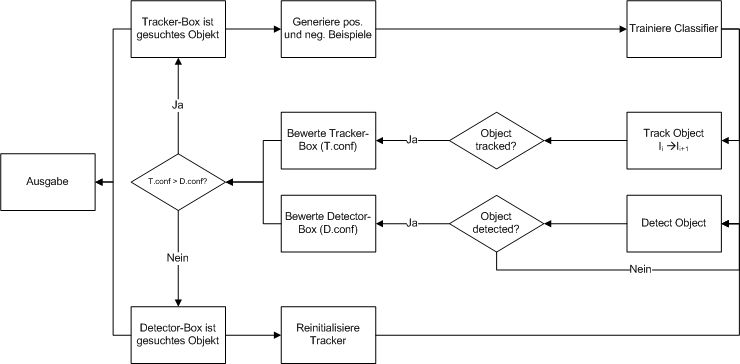
\includegraphics[scale=0.5]{../pictures/PAP.png}
	\caption{Zusammenspiel der Komponenten im Programmablaufplan}
	\label{abb:pap}
	\end{figure}

	Prinzipiell ist für die Initalisierung von TLD eine Nutzereingabe erforderlich. Diese Dient einzig der Markierung des gesuchten Objekts. \label{subsection:working_components} Entweder wird in einem Ausgabebild das Objekt durch ein Rechteck markiert, oder ein bereits erzeugtes Model wird geladen, wordurch die Classifier mit den entsprechenden Datenbasen initialisiert werden. Ein dritte Möglichkeit biete eine vorgeschaltete Komponente, wie zum Beispiel ein alternativer Klassifizierer, der für die Erkennung eines bestimmten Objekts trainiert wird und die initialie BoundingBox liefert. Nachdem die Initialisierung durchgeführt wurde, arbeitet TLD selbständig und ohne weitere Eingaben von Außen. Die Tracking- sowie die Detection-Komponente arbeiten vollkommen unabhängig und parallel. Beide liefern nach der Abarbeitung ein Ergebnis in Form einer Box, die Kandidaten für das gesuchte Objekt sind. Aufgrund des Sliding-Window-Ansatzes und des abschließenden Clusterings ist es möglich, dass der Detector mehr als eine mögliche Box als Ausgabe bestimmt, also kein eindeutiges Ergebnis liefert. In diesem Fall wird für die folgende Bewertung nur die Box des Trackers berücksichtigt, und die Ergebnismenge des Detectors wird verworfen.

	Liefern Detector und Tracker jeweils eine Box, wird mittels NearestNeigbour-Classifier bestimmt, welche der beiden Boxen am Ehesten dem gesuchten Objekt entspricht. Die berechneten Werte sind $T.conf$ für den Confidense-Value des Trackerergebnisses beziehnungsweise $D.conf$ für den Confidense-Value des Detectorergebnisses.

	\paragraph{$T.conf\geq D.conf$}
	Die Box des Trackers hat einen höheren Confidense-Value als die des Detectors. Das bedeutet, dass die Classifier, die Teil des Detectors sind, das Objekt in seiner gefundenen Form nicht erkannt habe, was wiederum bedeutet, dass neue Beispiele generiert werden müssen. Der Trainingsprozess wird angestoßen, die synthetischen positiven Beispiele werden generiert und der Lernfunktion übergeben. Diese bewertet wiederum jedes Beispiel mittels des NearsestNeighbour-Classifier und wenn es ``zu gut'' ist, das heißt $conf\geq.65$, wird das Beispiel verworfen.

	\paragraph{$T.conf<D.conf$ }
	Der Detector liefert das bessere Ergebnis, was wiederum bedeutet,	dass der Tracker das Objekt nicht finden konnte, weil es verdeckt oder teilweise nicht sichtbar war, oder der Tracker gedrifftet ist. In jedem Fall wird der Tracker mit der Detector-Box reinitalisiert. Ein Training findet in diesem Fall nicht statt.

	\subsection{Initialisierung}
	\label{subsection:tld_init}
	Wie bereits in bei \ref{subsection:working_components} erwähnt, gibt es verschiedene Möglichkeiten TLD zu initialisieren. Einzig die Repräsentation des Objekts mittels BoundingBox mit gewährleistet sein. Da die Kopter sich automatische gegenseitig erkennen sollen und kein weiterer Objekt-Detector als TLD implementiert werden soll, wird initial ein bereits erzeugtes und trainiertes Modell eine Kopters geladen. Der Ablauf des Trainings wird in \ref{subsection:learning_and_testing} näher erläutert. % Tracking-Learning-Detection TLD
		\cleardoublepage % -*- root: diplomarbeit.tex -*-
\section{Implementierung und Testszenarien}
Das folgende Kapitel behandelt den praktischen Teil der Diplomarbeit. Es werden die Implementierung in C++ beschrieben, die erzeugten Klassen vorgestellt sowie auf eventuelle Probleme und Besonderheiten während der Entwicklung eingegangen. Im Anschluss folgte die Beschreibung der verwendeten Testszenarien sowie die Erläuterung der durchgeführten Lernphasen.

\subsection{Programmierung}
Die Implementierung erfolgte in C++. Zusätzlich wurden OpenCV als unterstützendes Framework genutzt. Die grundlegende Klassenstruktur ist in Abbildung \ref{klassendiagramm} verdeutlicht.

\begin{figure}
\begin{centering}
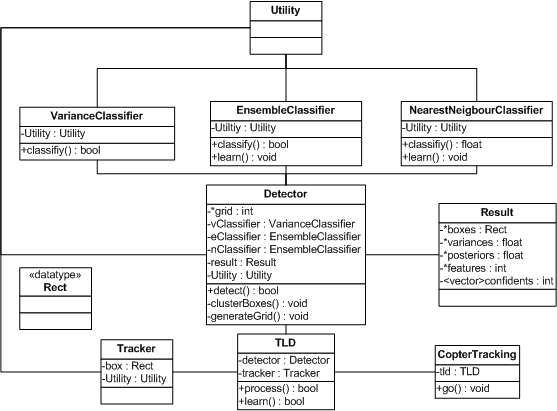
\includegraphics{../pictures/Klassendiagrammvsd.jpg}
\caption{Klassendiagramm zur Implementation mit den wichtigsten Attributen und Methoden}
\label{klassendiagramm}
\par\end{centering}
\end{figure}

\subsubsection{Klassenstruktur}
\paragraph{Klasse \textit{CopterTracking}}
Sie bildet den Einstieg in das Programm. Mittels OpenCV wird das Kamera- beziehnungsweise Videobild Frame für Frame eingelesen. Außerdem erfolgt hier die Definition des Objekts und die Übergabe des nächsten zu analysierenden Bildes sowie der Objektrepräsentation durch die aktuelle Box an die Klasse \textit{TLD}.

\paragraph{Klasse \textit{TLD}}
Diese Klasse definiert den eigentlichen Algorithmus und implementiert alle Methoden für das Zusammenspiel der Tracking-Detection-Learning-Komponenten. Kernstück bildet die Funktion \textit{process()}, die als Eingabe das aktuelle Bild $I$ mit der zuletzt gefundenen BoundingBox $b$ erwartet und die BoundingBox $b'$ berechnet und zurück liefert, sofern das Objekt gefunden wird. Neben der Initialisierung aller Komponenten beim Start des Programms, implementiert sie auch die Auswertung der Ergebnismengen von Tracker und Detektor in \textit{compareBoundingBoxes()}, die beide unabhängig von einander die Daten verarbeiten. Das ist die Implementierung von P-N Learning (3.3).

\paragraph{Klasse \textit{Tracker}}
Die Implementierung des MedianFlow-Trackers ist in dieser Klasse realisiert.

\paragraph{Klasse \textit{Detector}}
Diese Klasse implementiert die Kaskade aus den drei Classifiern \textit{Variance Classifier}, \textit{Ensemble Classifier} und \textit{NearestNeigbour Classifier}. Weiterhin sammelt der Detektor alle Ergebnisse zum gesuchten Kopter als \textit{Result}-Objekt und berechnet in der Funktion \textit{clusterBoxes()} die Cluster, aus denen dann ein oder mehrere finale Boxen berechnet werden. Initial definiert der Detektor mittels der Funktion \textit{generateGrid()} das \textit{Grid} als eine \textbf{int}-Zeigervariable, die Grundlage des sliding-window-Ansatzes ist. Es hat sich während der Implementierung gezeigt, dass eine Indexierung auf einer Zeigervariable die Abarbeitungsgeschwindigkeit gegenüber einer Implementierung des Grids in Form eines Vektor-Objekts stark erhöht.

\paragraph{Klasse \textit{Variance Classifier}}
In einer Schleife werden nacheinander alle durch das \textit{Grid} gegebene Windows mittels Klassifizierer-Kaskade bewertet. Die erste Stufe, bildet die Klasse Variance Classifier. Die Methode \textit{classify()} zeichnet sich für die Bewertung verantwortlich und füllt die entsprechenden Varianz-Werte des \textit{Result}-Objekts.

\paragraph{Klasse \textit{Ensemble Classifier}}
Stufe zwei der Kaskade ist durch die Klasse \textit{Ensemble Classifier} definiert, die im Detail den vorgestellten \textit{Fern Classifier} repräsentiert. Auch diese hat eine \textit{classify()}-Methode, verfügt jedoch zusätzlich über eine \textit{learn()}-Methode, mit die der Klassifizierer in der Lernphase trainiert wird.

\paragraph{Klasse \textit{NearestNeigbour Classifier}}
Die letzte Stufe ist der \textit{NearestNeigbour Classifier} mit den zur Klassifizierung und zum Trainieren benötigten Methoden \textit{classify()} und \textit{learn()}. Neben der Nutzung im Detektor dient er auch zur Bewertung der Tracker- und Detektor-Box durch die \textit{P-N Learning}-Komponente in der \textit{TLD}-Klasse für die Lernphase.

\paragraph{Klasse \textit{Result}}
Während der Bewertung jeder einzelnen Box durch die Kaskade der drei Classifier, werden neben der eigentlichen Klassifizierung, auch die ermittelten Werte (variance, posteriors, confidence) und die durch ein Rechteck definierte Box in dem \textit{Result-Objekt} zwischengespeichert. Die berechneten Werte werden in Zeiger- beziehungsweise Vektor-Variablen gespeichert. Vor allem erstere bieten einen sehr schnellen Speicherzugriff und damit eine laufzeitstarke Abarbeitung von TLD.

\paragraph{Klasse \textit{Utility}}
Diese Klasse liefert eine Reihe Klassenmethoden für unterschiedliche Berechnungen, die an verschiedenen Stelle im Programm genutzt werden.

\paragraph{Zusätzliche Angaben}
In den ersten Versionen des Programms wurde ein streng objektorientierter Ansatz verfolgt. Das bedeutet, dass das Objekt-Modell auch als eine solche Klasse definiert war. Und alle Objekte bildeten wiederum eine Grid, das als Vektor-Variable hinterlegt war. Wie sich allerdings gezeigt hat, war die Abarbeitungsgeschwindigkeit bei einem großen Grid und damit einer Menge von Objekten nicht zufriedenstellend. Trotz Übergabe des Grids als call-of-reference-Zeigervariable war nur mit einer kleinen Gridgröße von maximal 4000 einzelnen Objekten eine passable Abarbeitung möglich. Dies entsprach allerdings bei weitem nicht der in der originalen MATLAB-Implementierung beschriebenen circa 50.000 Boxen. Indexierungen über Zeigervariablen sind um ein Vielfaches schneller und deshalb wurde ein Refactoring durchgeführt, in dem alle laufzeitkritischen Vektor-Variablen durch Zeiger ersetzt wurden. Die Herausforderung bestand im Anschluss darin, eine möglichst geschickte Indizierung zu erzeugen, da zum Teil mehrdimensionale Werte in einer eindimensionalen Variable hinterlegt werden müssen.

\subsection{Lern- und Testphasen}
\label{subsection:learning_and_testing}
Die Ergebnisse der originalen Implementation von TLD in Matlab sind beeindruckend und können in \cite{TLD} nachgelesen werden. In den meisten der genutzten Datensätze erreichte die TLD-Implementation zu jeden vergleichbaren Algorithmus hinsichtlich der definierten Kriterien die besten Ergebnisse. Diese Arbeit behandelt neben der Implementierung von TLD die Nutzung des Ansatzes für das Kopter-Tracking. Allgemeine Datensätze sind zur Bewertung der Resultate deshalb nicht geeignet. Deshalb wird auf einen weiteren Vergleich der in \cite{TLD} beschriebenen Art verzichtet.

\begin{figure}[H]
	\begin{centering}
		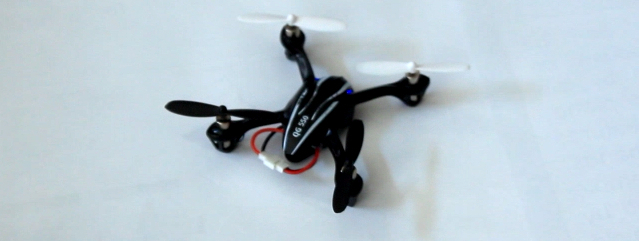
\includegraphics[scale=0.6]{../pictures/kopter}
		\caption{Das repräsentative Koptermodell MINI-QUADROCOPTER QG 550 XS für die Durchführung aller Tests.}
		\label{abb:kopter}
		\par
	\end{centering}
\end{figure}

Nach der Implementation sollte die Eignung von TLD auf das Koptertracking getestet werden. Dazu werden verschiedene Testszenarien erstellt, die nun kurz vorgestellt werden.

Als Datenquelle dienen in erster Linie Video- und Kamerasequenzen, die mittels einer handelsüblichen digitalen Spiegelreflexkamera beziehungsweise einer Standard Webcam in einer Auflösung von $640\times480$ Pixel aufgenommen sind. Als Modell wird der \textit{MINI-QUADROCOPTER QG 550 XS} gewählt (Abbildung \ref{abb:Kopter}). Die Testplattform für die Ausführung von TLD und der Durchführung der Tests ist ein \textit{DELL Studio 1555 Laptop} mit einem \textit{Intel(R) Core(TM)2 Duo Prozessor P8600, $2.40$Ghz} und \textit{6,00 GB RAM}. Es sollten vor allem zwei wesentliche Dinge überprüft werden:

\begin{enumerate}
\item Unter welchen Umständen beziehungsweise welche Kriterien müssen erfüllt werden, damit ein Kopter erfolgreich gefunden und verfolgt werden kann?
\item Kann durch spezielle Lernphasen und damit einer Verfeinerung des Models der Erfolg des Trackens verbessert werden?
\end{enumerate}

Da TLD bereits durch verschiedene, zum Download zur Verfügung stehende Evaluierungssequenzen getestet worden ist, und es für den speziellen Fall des Kopter-Trackings keine Daten vorhanden waren, wurden ausschließlich eigene Sequenzen verwendet.

\subsubsection{Videosequenzen}
Die verwendeten Videosequenzen decken Szenarien ab, in denen ein Kopter getrackt werden muss. Es werden verschiedene mögliche negative Einflussfaktoren wie Änderungen der Lichtverhältnisse, wechselnde Bewegungsgeschwindigkeiten und Bewegungsrichtungen mit Innen- und Außenaufnahmen simuliert. Neben der manuellen Initialisierung von TLD durch den Nutzer, dienten die in den Szenen erzeugten Models in einigen Testläufen ebenfalls als Initialisierung und wurden zusätzlich erweitert.

\subsubsection{Kamerasequenzen}
Da Videosequenzen nur bedingt für die Verfeinerung eines Models geeignet sind, wurden zusätzlich Kamerasequenzen genutzt. Dadurch kann auf Tracking-Detection-Probleme und der Verfälschung des Models durch fehlerhafte Fokussierung von TLD reagiert werden.

\begin{figure}[H]
  \begin{centering}
    %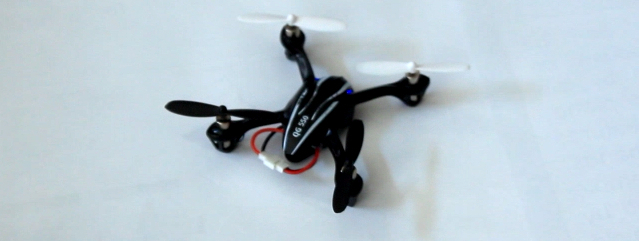
\includegraphics[scale=0.6]{../pictures/kopter}
    HIER EIN PAAR SEQUENZEN.
    \caption{Die Sequenzen als Datensätze. BESCHREIBUNGEN}
    \label{abb:sequenzen}
    \par
  \end{centering}
\end{figure} % Implementierung und Testszenarien
		\cleardoublepage % -*- root: diplomarbeit.tex -*-
\section{Auswertung und Ausblick}
	Object Detection ist eines der herausfordernsten Forschungsfelder in Computer Vision. Obwohl die Entwicklung von robusten und gut funktionierenden Ansätzen in den letzten Jahren stark zugenommen hat und unter kontrollierten Bedingungen auch sehr gute Ergebnisse liefert, ist das Problem des Suchens und Findesn von einem oder mehreren Objekten in der ``realen'' Welt weiterhin ungelöst \cite{ODS}.

\subsection{Evaluation}
	Die Evaluation von TLD erfolgt mit Hilfe eine Standardverfahrens zur Beurteilung von Klassifikatoren und findet auch in \cite{TLD}. Hierbei dienen die quantitativen Ergebnisse des Klassifizierers in jedem Testszenario als Maß. Da TLD ein binärer Klassifizier ist, gibt es zwei Arten von Fehlern die auftreten können. Entweder wird das Objekt in die Klasse $A$ eingeordnet, obwohl es zu $B$ gehört, oder es wird als Teil von $B$ bestimmt, gehört allerdings zur Klasse $A$. $A$ und $B$ sind in Falle von TLD ``gefunden'' und ``nicht gefunden''.
	
	Als Vergleichsbasis dient der Ground Truth. Das ist der Bereich, der die genaue Position des gesuchten Kopters im Bild markiert, gegeben durch eine BoundingBox $BB_{GT}$. Dieser wird mit dem Ergebnis von TLD verglichen, der ebenfalls eine BoundingBox $BB_{TLD}$ bei erfolgreicher Detection beziehnungsweise erfolgreichem Tracking liefert. Zwischen beiden Boxen wird die Überlappung bestimmt und geprüft, ob sie größer oder kleiner eines Thresholds $\omega$ ist. Daraus ergeben sich vier Fälle:

	\begin{description}
		\item [True-Positive $t_p$] Die Überlappung ist größer als $\omega$.
		\item [True-Negative $t_n$] Es wurde kein Objekt gefunden und es wurde auch keines erwartet.
		\item [False-Positive $f_p$] Der Algorithmus findet ein Objekt, obwohl keines erwartet wurde, oder die Überlappung ist kleiner als $\omega$.
		\item [False-Negative $f_n$] Der Algorithmus findet kein Objekt, obwohl eines erwartet wurde, oder die Überlappung ist kleiner als $\omega$.
	\end{description}

	In jedem Testdurchlauf werden die Anzahl $t_p$, $t_n$, $f_p$ und $f_n$ gezählt und mittels statistischer Gütekriterien ausgewertet. 
  Wie auch bei \cite{TLD} sind diese Kriterien Genauigkeit (Precision) \begin{equation} P=\frac{t_p}{(t_p + f_p)},\end{equation}
  Trefferquote (Recall) \begin{equation} R=\frac{t_p}{(t_p + f_n)} \end{equation}
  und das gewichtete harmonische Mittel \begin{equation} F=\frac{2 \times (P \times R)}{(P + R)}.\end{equation}

  HIER WEITER!!!

\subsection{Resultate}
	Hier kommen die Resultate der Testreihen 

\subsection{Auswertungen und Beobachtungen} 
	\label{subsec:conclusion}
	TLD beeindruckt durch sehr gute Ergebnisse beim Tracken von unterschiedlichen Objekten, wie Fußgänger, Autos und Gesichtern \cite{TLD}. Als Detectionstrategie ist dieser semi-supervised-learning-Ansatz für eine Vielzahl von Fällen geeignet. Die natürlich gegebenen Umwelteinflüsse wie zum Beispiel unterschiedliche Beleuchtungen der Szenerie durch Licht-Schatten-Wechsel werden durch die Detectorkaskade gut verarbeitet. Wie die Resultate jedoch verdeutlichen, ist TLD trotz der vielen Stärken für die Koptererkennung nur bedingt leistungsfähig. Die Gründe werden im Folgenden vorgestellt und analysiert.

	\paragraph{Detectorkaskade}
	Die letzte Komponente der Detectorkaskade, der Nearest-Neighbour-Classifier, speichert Patches des Objekts in der Größe $15\times15 px$. Bestimmt durch die BoundingBox wird meist auch ein Teil des Hintergrundes gespeichert und gelernt. Somit ist nicht nur das Objekt selbst, sondern auch seine Umgebung Teil der Repräsentation. Der Einfluss ist hierbei stark von Größe und Beschaffenheit des Objekts sowie der Menge an ``Hintergrund'', der gespeichert wird, abhängig.

	Ein Kopter wird durch einen anderen Kopter meist von der Seite wahrgenommen. Aufgrund der dünnen/kompakten/filigranen Struktur wird unweigerlich immer eine Menge Hintergrundinformationen im Patch gespeichert (Abbildung \ref{abb:problem_background_1}). Der Einfluss auf die Genauigkeit und die Trefferquote des Detectors ist damit sehr groß. Probleme treten vor allem dann auf, wenn der Hintergrund einen hohen Informationsgehalt hat, wie zum Beispiel Bäume oder Häuser, da der Kopter selbst strukturell eher einfach aufgebaut ist. Aber auch Hintergründe mit unterschiedlichen Farbstärke sind problematisch. So kann es vorkommen, dass ein Kopter, dessen Model vor einem hellen Hintergrund ``erlernt'' wurde, vor einem dunklen nicht mehr erkannt wird. 

	Um den Einfluss des Hintergrundes zu minimieren, ist es möglich nur einen Teil des Kopters initial zu markieren, wie zum Beispiel den Corpus ohne die Rotoren (Abbildung \ref{abb:problem_background_2}). Das führt allerdings dazu, dass der Kopter ausschlielich anhand dieses Teilbereichs erkannt wird, also nur von einer Seite. Das macht es unmöglich eine vollständiges Model des Objekts zu generieren.

	\begin{figure}
		\begin{centering}
			% 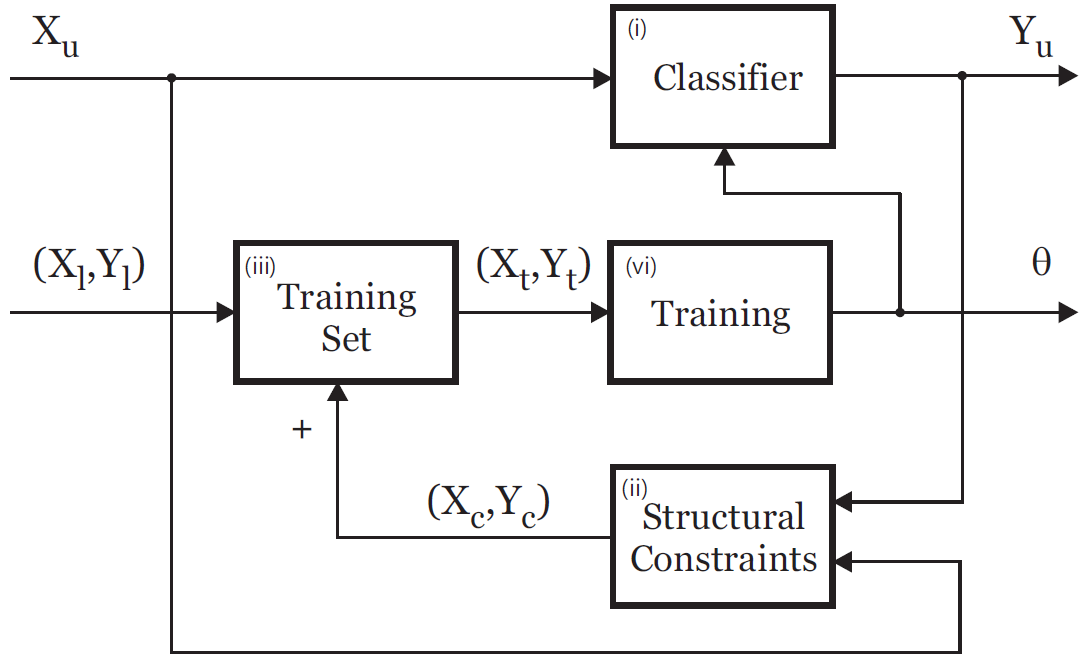
\includegraphics[scale=0.4]{../pictures/PN_LEARNING.png}
			(BILD MIT KOPTER UND BOUNDINGBOX UND VIEL HINTERGRUND)
			\caption{Problem: Detector 1}
			\label{abb:problem_background_1}
			\par
		\end{centering}
	\end{figure}

	\begin{figure}
		\begin{centering}
			% 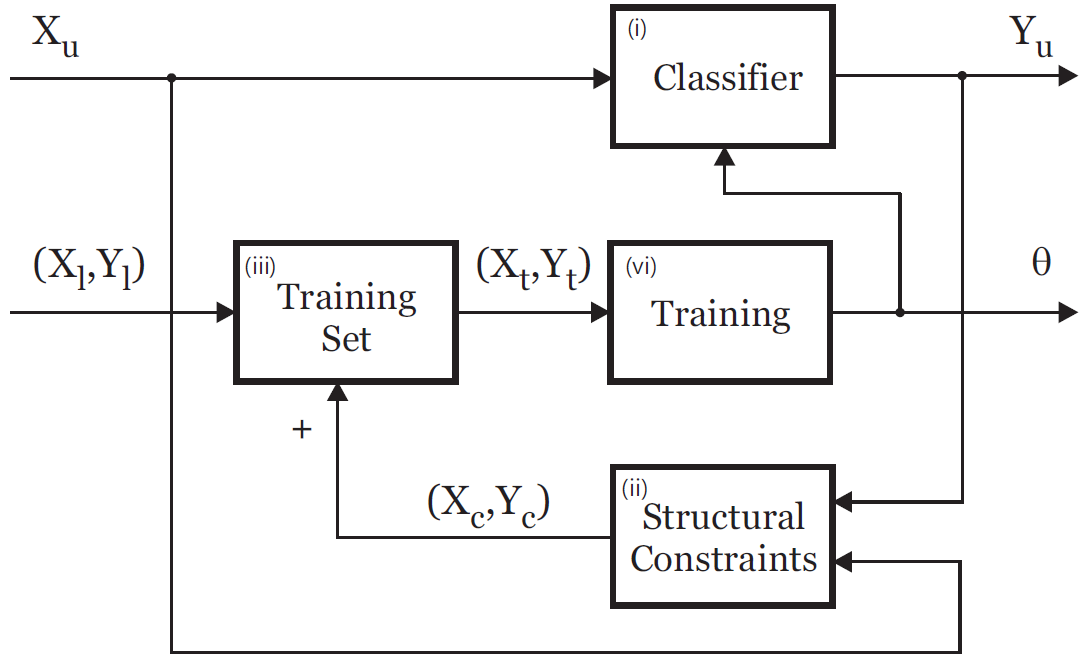
\includegraphics[scale=0.4]{../pictures/PN_LEARNING.png}
			(BILD MIT KOPTER UND BOUNDINGBOX UND KEINEM HINTERGRUND)
			\caption{Problem: Detector 2}
			\label{abb:problem_background_2}
			\par
		\end{centering}
	\end{figure}
	
	

	\paragraph{MedianFlow Tracker}
	Die Struktur des Kopters bedingt nicht nur den Erfolg des Detectors, sondern beeinflusst ebenfalls die Leistung des Trackers. Dieser schätzt anhand einer regelmäßigen Anordnung von Punkte innerhalb einer BoundingBox in einem Frame, die Position der Punkte im Folgebild. Diese regelmäige Anordnung ist gleichförmig, wodurch viele Punkte, die zum Hintergrund gehören, die LKT-Schätzung beeinflussen (Abbildung \ref{abb:problem_tracker}). Auch hier stellen vor allem detailreiche Hintergründe ein Problem dar, weil durch die willkürliche Wahl der Punkte die Wahrscheinlichkeit erhöht wird, eine ungenaue Schätzung zu erhalten.

	\begin{figure}
		\begin{centering}
			% 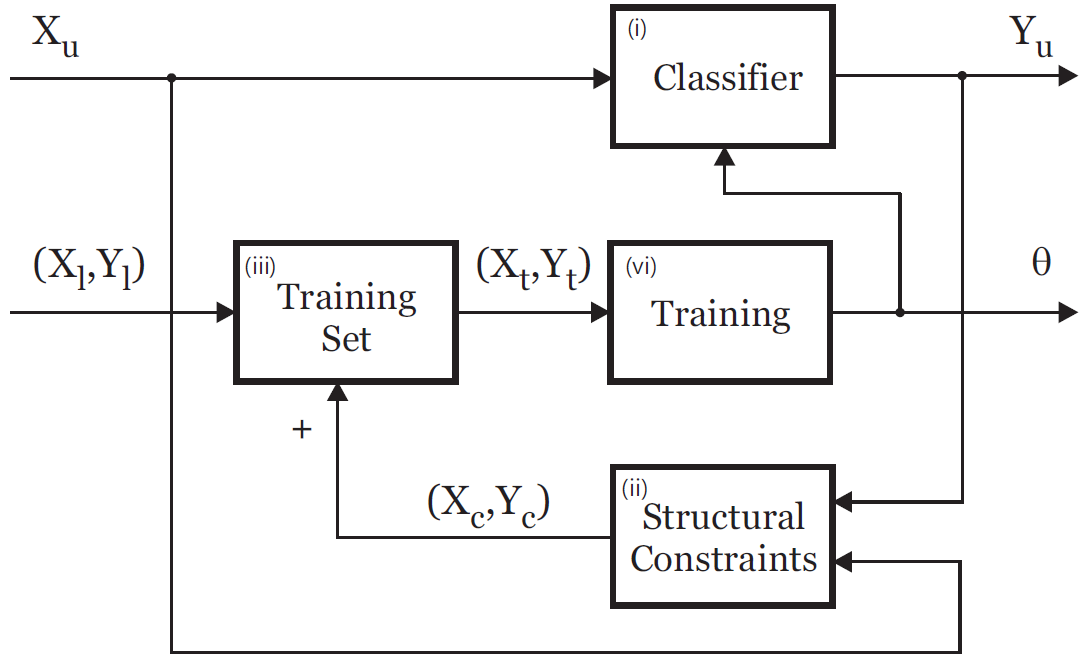
\includegraphics[scale=0.4]{../pictures/PN_LEARNING.png}
			(BILD MIT PUNKTEN UND HINTERGRUND FÜR TRACKER)
			\caption{Problem: Tracker}
			\label{abb:problem_tracker}
			\par
		\end{centering}
	\end{figure}

	Ein zusätzlicher Nachteil des Trackers ist, dass er keine Lernkomponente besitzt. Jede Verarbeitung ist unabhängig und integriert keine zusätzlichen Informationen aus vergangenen Schätzungen, was bedeutet, dass der Tracker immer wieder die gleichen Fehler macht - im Gegensatz zum Detector, der aus seinen Fehlern ``lernt''. 

	% Der Ansatz ist nur bedingt geeignet. Probleme:
	% \begin{itemize}
	% \item Speichern der Beispiele in Form von $15\times15$ patches, weil zu viel Hintergrund gespeichert wird,
	% \item Objekt (Kopter) hat filigrane Struktur,
	% \item ``Veschmelzung'' des Objekts mit dem Hintergrund
	% \end{itemize}
	% Weiteres...
	% \begin{itemize}
	% \item Ein paar Worte zur Umsetzung (openCV)
	% \item Erweiterungsmöglichkeiten - z.B. Verfolgung mehrerer Kopter gleichzeitig, Optimierungsvorschläge, weitere Einsatzmöglichkeiten (da TLD an sich ``alles'' tracken kann)
	% \item Zusammenfassung
	% \item ohne zusätzlich Detectionsverfahren (eventuell Tiefenbilder oder andere nicht-visuelle Ansätze) kaum möglich
	% \item Umwelteinflüsse in der Natur sind zu stark
	% \item Einfluss der unterschiedlichen Beleuchtungen der Szene
	% \item Hintergrund (Bäume etc)
	% \item Problem bei zusätzlichen Verfahren: Rechenleistung des Roboters(?)
	% \end{itemize}

\subsection{Modikfikationen und Verbesserungsvorschläge}
	Die strickte Trennung der einzelnen Komponenten in TLD bietet die Möglichkeit eine Reihe von Änderungen vorzunehmen, ohne die prinzipielle Arbeitsweise zu verändern. Das ist eine zusätzliche Stärke des Algorithmus. Im folgenden Abschnitt werden Modifikationen diskutiert, die TLD für die Koptererkennung leistungsfähiger machen können.

	\paragraph{Detectorkaskade}
	Neben der in \cite{TLD} diskutierten Vorschläge, wie zum Beispiel einen Forground Filter, der allerdings in dieser Arbeit sicherlich keine signifikanten Verbesserungen nach sich ziehen würde, gibt es weitere Anpassungen der Detector-Komponente, die hier diskutiert werden.

	Wie in \ref{subsec:conclusion} erläutert, ist die Datenbasis des Nearest-Neigbour-Classifier für die Koptererkennung nicht gut geignet. Die Struktur des Objekts bedingt das Speichern von zu vielen Hintergrundinformationen, was die Berechnung des $conf$-Wertes und damit die Klassifikation stark negativ beeinflusst. Ein andere Repräsentation, eventuell mit herausgefiltertem Hintergrund oder einer anderen Speicherform als Patch wäre sinnvoll.

	\paragraph{MedianFlow Tracker}
		Zum einen könnte die Tracker-Komponente mit einem anderen Verfahren die Punkte für die Schätzung wählen. Eventuell würde eine nicht gleichförmige Verteilung der Punkte innerhalb der BoundingBox die Genauigkeit erhöhen und die Fehleranfälligkeit verringern. Eine Verringerung der Punktedichte vom Zentrum aus zu den Rändern der Boxwürde den Einfluss Hintergrunds auf das Ergebnis verringert.

		Das Ersetzen der MedianFlow Trackers durch eine andere Komponente wäre ebenfalls möglich. Trackingimplementationen mittels \em{Kalman-Filter} \cite{KAF} oder \em{Particle-Filter} \cite{PAF} liefern sehr gute Ergebnisse [Quelle]. Anstelle der Punktrepräsentation wären eine Objektdefinition anhand der Form oder segnifikanter Linien denkbar und wurden auch bereits erfolgreich eingesetzt \cite{AVT}. 

	\paragraph{Allgemein}
		Der Kopter soll selbst sein bestes Modell darstellen, weshalb als Vorgabe gilt, dass keine Modifikationen an ihm vorgenommen werden dürfen. Dazu gehören Markierungen jeglicher Art, wie zum Beispiel Farb- oder Musterapplikationen. Deshalb wurde TLD für die Implementation gewählt, weil die Verarbeitung grundsätzlich mit jedem Objekttyp funktioniert und keine speziellen Modifikationen am Objekt nötig sind. Wie die Resultate und die Auswertung zeigen, ist diese Restriktion jedoch zu stark, denn der Kopter selbst ist nicht signifikant genug, um sich von seiner Umgebung ausreichend abzuheben. Die Verarbeitung zusätzlicher Informationen zur Verbesserung der Lösung ist anzuraten und wird kurz präsentiert.

		TLD arbeitet prinzipiell farbunabhängig, die Berechnung erfolgt einzig auf Grauwertbildern, könnten spezielle Markierungen auf den Flugrobotern die Ergebnisse verbessern. Ähnlich wie beim Robocup, wo eine signifkante Kombination eines horizontalen Streifenmusters zum Beispiel die Spielbegrenzung markiert, wären eine ähnliche Vorgehensweise bei der Markierung der Kopter denkbar. Wenn dieses Muster Teil der Objektrepräsentation ist, wird der Kopter signifikanter und hebt sich besser von seiner Umgebung ab. 

		Eine Implementierung zur Verarbeitung von Farbbildern wäre ebenfalls eine Möglichkeit die Leistungsfähigkeit zu verbessern. Dazu müssen allerdings die im Allgemeinen uniformen Kopter farblich markiert werden, was wiederum den Restriktionen widerspricht. 

% Verbesserungen/Ansätze
% \begin{itemize}
% \item eventuell stärke Orientierung an natürlich Seh-prozessen bzw. Sensoren in der Natur (Auge der Fliege)
% \item Eventuell ein anderer Ansatz: Vielleicht sollte man eine 3-D Repräsentation des Objekts während des Trackens erzeugen? Der Mensch macht es sicher auch nicht anders. Schließlich weiß man ja oft, wonach man suchen muss, auch wenn das Erscheinungsbild des Objekts nicht mit dem bereits ``Erlernten'' übereinstimmt...
% \item Articulated shape models > hierbei werden Teile des Objekts einzeln repräsentiert und zu einem ganzen Zusammengesetzt. 
% \item Eventuell nicht so allgemeine Ansätze, sondern vorher viel mehr Wissen über das Objekt, den Kopter, als Grundlage nehmen. Eventuell ein 3- -Modell erzeugen und aus dem ermittelten Bild alle entsprechende Objekte auf dieses ``mappen''. 
% \end{itemize} % Auswertung Ausblick
		\cleardoublepage % -*- root: diplomarbeit.tex -*-
\section{Anhang}
\subsection*{OpenCV}
Die \textit{Open Source Computer Vision Library} OpenCV ist einen Bibliothek mit einer Sammlung von Klassen und Algorithmen in den Bereichen des machinellen Sehens, der Bildverarbeitung und des maschinellen Lernens implementiert und zur (meist) freien Verfügung stellt. Wurde anfangs nur die Sprache C unterstützt, gibt es heute ein Reihe von Implementierungen in C++, Python, Java und auch MATLAB. Außerdem werden sowohl die gängigen Betriebssysteme Windows, Linux und Mac OS, als auch das mobile OS Android unterstützt.

Zur Zeit befinden sich spezielle Module in der Entwicklung (basierend zum Beispiel auf CUDA), die es erlauben, Algorithmen expliziet auf der GPU (\textit{Graphic Processor Unit}), also auf dem Grafikprozessor, auszuführen. Die Auslagerung auf die für die Verarbeitung von Bilddaten optimierte Hardware hat vor allem Ge- schwindigkeitsvorteile (siehe Abbildung \ref{GPU_Performance}).

\begin{figure}
\centering{}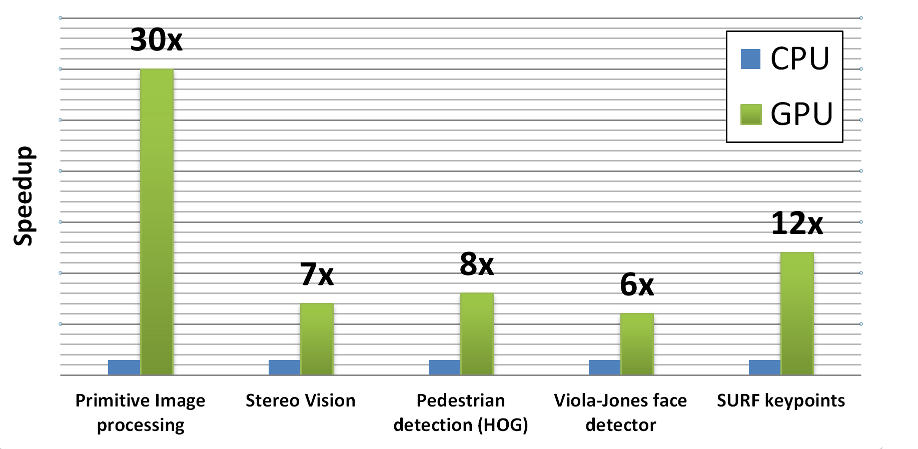
\includegraphics[scale=0.5]{../pictures/GPU_Performance.png}\caption{Tesla C2050 versus Core i5-760 2.8Ghz, SSE, TBB \cite{OCW}}
\label{GPU_Performance}
\end{figure}

\subsection*{OpenTLD}
Im Laufe der Bearbeitung des Themas wurde eine C++-Implementierung von TLD veröffentlicht. OpenTLD adaptiert die originale Matlab-Version, erweitert allerdings die Detector-Kaskade um einen weiteren Filter, den Foreground-Filter. Dieser dient in erster Linie zur Reduzierung der möglichen BoundingBoxes durch Subtraktion des Hintergrundes.

Mit Hilfe eines Forground-Filters kann ein sich bewegendes Objekt mittels Background-Substraction aus einer Videosequenz separiert werden{[}QUELLE{]}. Dieses Verfahren wird vor allem bei statischen Kameras verwendet, die fest montiert. In einer sehr dynamischen Anwendung, wie das Finden und Verfolgen von sich bewegenden Objekten mittels auf einem Flugroboter montierten Kamera unter Nichtlaborbedingungen, hat eine solche Komponente somit keine Relevanz auf die Robustheit des Algortihmus. Außerdem ist dieser Filter nicht Teil der originalen Veröffentlichung von Z. Kalal. Aus diesen Gründen wurde auf eine Implementierung verzichtet. Teile von OpenTLD wurden zu Analysezwecke und standen zur Vervollständigung der eigenen Implementierung Pate.

\subsection*{Algorithmen}
An dieser Stelle gibt es eine Übersicht der restlichen verwendeten Algorithmen.

\paragraph{Varianz-Classifier}
Hier die Erklärung des Algorithmus.

\begin{algorithm}[H]
	\vspace{0.2cm}
	\KwData{Input} 
	\KwResult{Output}
	TODO
	\caption{Varianz-Classifier}
	\label{alg:varianz}
	\vspace{0.2cm}
\end{algorithm}

\paragraph{Ensemble-Classifier}
Hier die Erklärung des Algorithmus.

\begin{algorithm}[H]
	\vspace{0.2cm}
	\KwData{Input} 
	\KwResult{Output}
	TODO
	\caption{Ensemble-Classifier}
	\label{alg:ensemble}
	\vspace{0.2cm}
\end{algorithm}

\paragraph{NearestNeighbour-Classifier}
Hier die Erklärung des Algorithmus.

\begin{algorithm}[H]
	\vspace{0.2cm}
	\KwData{Input} 
	\KwResult{Output}
	TODO
	\caption{NearestNeigbour-Classifier}
	\label{alg:nearest_neighbour}
	\vspace{0.2cm}
\end{algorithm}

\paragraph{Clustering}
Hier die Erklärung des Algorithmus.

\begin{algorithm}[H]
	\vspace{0.2cm}
	\KwData{Input} 
	\KwResult{Output}
	TODO
	\caption{Clustering}
	\label{alg:cluster}
	\vspace{0.2cm}
\end{algorithm}






 % Anhang
		\cleardoublepage % -*- root: diplomarbeit.tex -*-
\newpage{}

\begin{thebibliography}{SMAT}
\bibitem[TLD]{TLD} Z. Kalal, k. Mikolajczyk, and J. Matas. Tracking-Learning-Detection. \textit{Pattern Analysis and Machine Intelligence}, IEEE Transactions on (Volume:34 , Issue: 7 ), pages 1409-1422, July 2012

\bibitem[MFT]{MFT} Z. Kalal, k. Mikolajczyk, and J. Matas. Forward-Backward Error: Automatic Detection of Tracking Failures. \textit{Proc. 20th Int'l Conf. Pattern Recognition}, pages 23-26, 2010.

\bibitem[OPT]{OPT} Bruce D. Lucas and Takeo Kanade. An iterative image registration technique with an application to stereo vision. \textit{International Joint Conference on Artificial Intelligence}, pages 674-679, 1981.

\bibitem[OCV]{OCV}G. Bradski and A. Kaehler. Learning OpenCV: Computer Vision with the OpenCV Library.\textit{ O\textquoteright{}Reilly Media, 1st edition}, Oct. 2008.

\bibitem[NCC]{key-5} J.P. Lewis. Fast normalized cross-crorrelation. \textit{Vision Interface. Canadian Image Processing and Pattern Recognition Society}, pages 120-123, 1995.

\bibitem[IIM]{key-6}P. Viola and M. Jones. Rapid object detection using a boosted cascade of simple features. In \textit{2001 IEEE Computer Society Conference on Computer Vision and Pattern Recognition. CVPR 2001}, volume 1, pages I\textendash{}511\textendash{}I\textendash{}518, Los Alamitos, CA, USA, Apr. 2001

\bibitem[VID]{key-7} Video Analyse - Therie and practice.

\bibitem[PYR]{key-8} Jean-Yves Bouguet. Pyramidal Implementation of the Lucas Kanade Feature Tracker : Description of the algorithm, \textit{Intel Corporation \textendash{} Microprocessor Research Labs}, 2002.

\bibitem[BAB]{BAB} M. B. Blaschko. Branch and Bound Strategies for Non-maximal Suppression in Object Detection, volume 6819 of Lecture Notes in Computer Science, chapter 28, pages 385\textendash{} 398. Springer Berlin Heidelberg, Berlin, Heidelberg, 2011.

\bibitem[OTS]{OTS} A. Yilmaz, O. Javed, and M. Shah, Object tracking: A survey. \textit{ACM Computing Surveys (CSUR)}, vol. 38, no. 4, 2006.

\bibitem[PNL]{PNL}Z. Kalal, J. Matas, and K. Mikolajczyk. P-N learning: Bootstrapping binary classifiers by structural constraints. In \textit{2010 IEEE Conference on Computer Vision and Pattern Recognition (CVPR)}, pages 49\textendash{}56. IEEE, June 2010

\bibitem[ODS]{ODS}D.K.Prasad. Survey of The Problem of Object Detection In Real Images. \textit{In International Journal of Image Processing (IJIP)}, Volume (6) : Issue (6), pages 441 - 466, 2012

\bibitem[STV]{STV} B. D. Lucas and T. Kanade, \textquotedblleft{}An
iterative image registration technique with an application to stereo vision,\textquotedblright{} International Joint Conference on Artificial Intelligence, vol. 81, pp. 674\textendash{}679, 1981.

\bibitem[GFT]{GFT} J. Shi and C. Tomasi, \textquotedblleft{}Good features to track,\textquotedblright{} Conference on Computer Vision and Pattern Recognition, 1994.

\bibitem[KBT]{KBT}D. Comaniciu, V. Ramesh, and P. Meer, \textquotedblleft{}Kernel-Based Object Tracking,\textquotedblright{} IEEE Transactions on Pattern Analysis and Machine Intelligence, vol. 25, no. 5, pp. 564\textendash{}577, 2003.

\bibitem[TUP]{TUP}I. Matthews, T. Ishikawa, and S. Baker, \textquotedblleft{}The Template Update Problem,\textquotedblright{} IEEE Transactions on Pattern Analysis and Machine Intelligence, vol. 26, no. 6, pp. 810\textendash{}815, 2004

\bibitem[SMAT]{SMAT}N. Dowson and R. Bowden, \textquotedblleft{}Simultaneous Modeling and Tracking (SMAT) of Feature Sets,\textquotedblright{} Conference on Computer Vision and Pattern Recognition, 2005.

\bibitem[RDT]{RDT}A. Rahimi, L. P. Morency, and T. Darrell, \textquotedblleft{}Reducing drift in differential tracking,\textquotedblright{} Computer Vision and Image Understanding, vol. 109, no. 2, pp. 97\textendash{}111, 2008.

\bibitem[ROAM]{ROAM}A. D. Jepson, D. J. Fleet, and T. F. El-Maraghi, \textquotedblleft{}Robust Online Appearance Models for Visual Tracking,\textquotedblright{} IEEE Transactions on Pattern Analysis and Machine Intelligence, pp. 1296\textendash{}1311, 2003.

\bibitem[RFT]{RFT}A. Adam, E. Rivlin, and I. Shimshoni, \textquotedblleft{}Robust Fragments-based Tracking using the Integral Histogram,\textquotedblright{} Conference on Computer Vision and Pattern Recognition, pp. 798\textendash{}805, 2006.

\bibitem[ETR]{ETR}M. J. Black and A. D. Jepson, \textquotedblleft{}Eigentracking: Robust matching and tracking of articulated objects using a view-based representation,\textquotedblright{} International Journal of Computer Vision, vol. 26, no. 1, pp. 63\textendash{}84, 1998.

\bibitem[RVT]{RVT}D. Ross, J. Lim, R. Lin, and M. Yang, \textquotedblleft{}Incremental Learning for Robust Visual Tracking,\textquotedblright{} International Journal of Computer Vision, vol. 77, pp. 125\textendash{}141, Aug. 2007.

\bibitem[VTD]{VTD}J. Kwon and K. M. Lee, \textquotedblleft{}Visual Tracking Decomposition,\textquotedblright{} Conference on Computer Vision and Pattern Recognition, 2010.

\bibitem[ONS]{ONS}R. Collins, Y. Liu, and M. Leordeanu, \textquotedblleft{}Online Selection of Discriminative Tracking Features,\textquotedblright{} IEEE Transactions on Pattern Analysis and Machine Intelligence, vol. 27, no. 10, pp. 1631\textendash{}1643, 2005.

\bibitem[ENT]{ENT}S. Avidan, \textquotedblleft{}Ensemble Tracking,\textquotedblright{} IEEE Transactions on Pattern Analysis and Machine Intelligence, vol. 29, no. 2, pp. 261\textendash{}271, 2007.

\bibitem[OBT]{OBT}H. Grabner and H. Bischof, \textquotedblleft{}On-line boosting and vision,\textquotedblright{} Conference on Computer Vision and Pattern Recognition, 2006.

\bibitem[MIP]{MIP}Milan Sonka and J. Michael Fitzpatrick, Handbook of Medical Imaging : Medical Image Processing and Analysis Volume 2

\bibitem[LCD]{LCD}Tseng, D.-C., I-Ling Chung, Pei-Lin Tsai, and Chang-Min Chou, \textquotedbl{}Defect classification for LCD color filters using neural network-based decision tree classifier,\textquotedbl{} International Journal of Innovative Computing, Information and Control, vol.7, no.7 (A), pp.3695-3707, 2011.

\bibitem[PED]{PED}R. Benenson, M. Mathias, R. Timofte, and L. V. Gool, \textquotedblleft{}Pedestrian detection at 100 frames per second,\textquotedblright{} in Proc. IEEE Int\textquoteright{}l Conf. on Computer Vision and Pattern Recognition , 2012, pp. 2903\textendash{}2910.

\bibitem[OCW]{OCW}http://opencv.org/platforms/cuda.html, 29.09.2013

\bibitem[FPIS]{FPIS}SETHI, I. AND JAIN, R. Finding trajectories of feature points in a monocular image sequence. \textit{IEEE Trans. Patt. Analy. Mach. Intell. 9}, 1, 56\textendash{}73, 1987

\bibitem[KAF]{KAF}Kalman, R. E., A New Approach to Linear Filtering and Prediction Problems., \textit{Transactions of the ASME--Journal of Basic Engineering, Vol 82, Series D}, pp. 35 - 45, 1960 

\bibitem[PAF]{PAF} Gordon N.J., Salmond D.J. and Smith A.F.M., Novel approach to nonlinear/non-Gaussian Bayesian state estimation. \textit{IEE-Proceedings-F}, 140 , 107 - 113, 1993

\bibitem[INT]{INT} H., BELL, J. W., AND WU, F. 2002. Very fast template matching. \textit{In European Conference on Computer Vision (ECCV)}. 358\textendash{}372.

\bibitem[LKT]{LKT}Carlo Tomasi and Takeo Kanade. Detection and Tracking of Point Features. \textit{Carnegie Mellon University Technical Report CMU-CS-91-132}, April 1991.

\bibitem[BSGF]{BSGF} Dominik A. Klein and Armin B. Cremers, \textquotedblleft{}Boosting Scalable Gradient Features for Adaptive Real-Time Tracking, \textquotedblright{} \textit{IEEE Int. Conf. on Robotics and Automation (ICRA)}, pp. 4411-4416, May 2011

\bibitem[AVT]{AVT} D. A. Klein, D. Schulz, S. Frintrop and A. B. Cremers, Adaptive Real-Time Video-Tracking for Arbitrary Objects, \textit{IEEE Int. Conf. on Intelligent Robots and Systems (IROS)}, pp. 772-777, October 2010

\end{thebibliography} % Bibliographie
		\cleardoublepage % -*- root: diplomarbeit.tex -*-
\appendix
\thispagestyle{empty}
%%%%%%%%%%%%%%%%%%%%%%%%%%%%%%%%%%%%%%%%%%%%%%%%%%%%%%%%%%%%%%%%%%%%%%%%%%%%%%%%%%%%%%%%%%%%%%%%%%%% %% Selbststaendigkeitserklaerung %%%%%%%%%%%%%%%%%%%%%%%%%%%%%%%%%%%%%%%%%%%%%%%%%%%%%%%%%%%%%%%%%%%%%%%%%%%%%%%%%%%%%%%%%%%%%%%%%%%%
{\parindent 0cm      
\subsection*{Selbst\"andigkeitserkl\"arung}   
  Ich erkl\"are hiermit, dass ich die vorliegende Arbeit selbst\"andig verfasst    und nur unter Verwendung der angegebenen Quellen und Hilfsmittel angefertigt habe.    Weiterhin erkl\"are ich, eine Diplomarbeit in diesem Studiengebiet erstmalig einzureichen.\\ 

\vspace{3\baselineskip}      Berlin, den \today \hspace{0.25\linewidth}\parbox{0.3\linewidth}{\dotfill}
%%%%%%%%%%%%%%%%%%%%%%%%%%englische Version%%%%%%%%%%%%%%%%%%%%%%%%%%%%%%%%%%%%%%%%%%%%%%%%%%%%%%%%% \selectlanguage{english} 
\subsection*{Statement of authorship} 
  I declare that I completed this thesis on my own and that information which has been  directly or indirectly taken from other sources has been noted as such. Neither this  nor a similar work has been presented to an examination committee.

  \vspace{3\baselineskip} Berlin, \today
  \hspace{0.25\linewidth}\parbox{0.3\linewidth}{\dotfill} 
} % Eigenständigkeitserklärung
	\end{onehalfspace}
\end{document}